 \documentclass[a4paper,11pt,headings=standardclasses]{scrartcl}% see <http://www.komascript.de>
% ----------------------------------------------------------------------------
% font, style, etc.
\usepackage[utf8]{inputenc} % defines
\usepackage{csquotes}

% mathematics
\usepackage{amsmath}
\usepackage{amssymb}

% figures, tables, etc.
\usepackage{hyperref} %
\usepackage{graphicx}
\usepackage{tikz}
\usepackage{pgf}
\usepackage{xcolor}

% code
\usepackage{listings}
\lstset{
language=Python, 
backgroundcolor = \color{light-gray},
basicstyle=\scriptsize\sffamily,
stringstyle=\color{orange},
breaklines=true,
numberstyle=\tiny\color{gray},
keywordstyle=\bfseries\color{dark-blue}\textit, % print keywords dark-blue
commentstyle=\color{dark-green}, % print comments dark-green
showstringspaces=false} % spacing between strings not showed

% others
\usepackage{acronym}

% theorems
\newtheorem{defi}{Definition}[section]

% setup the appearance of links
\hypersetup{
    colorlinks = true, % false -> red box arround links (not very nice)
    linkcolor={red!20!black},
    citecolor={blue!50!black},
    urlcolor={blue!80!black},
}

% define shortcuts
\newcommand{\ad}{\mathrm{ad}}
\renewcommand{\d}{\mathrm{d}} % d vor differential forms
\newcommand{\NV}{{\cal N}\,}
\newcommand{\rang}{\mathrm{rang}}
\newcommand{\im}{\mathrm{im}}
\newcommand{\spann}{\mathrm{span}}
\newcommand{\R}{\mathbb{R}} %  set of real numbers
\newcommand{\py}{\emph{Python}\,}
\newcommand{\scipy}{\emph{SciPy}\,}
\newcommand{\mpl}{\emph{Matplotlib}\,}
\newcommand{\uu}{\mathbf{u}}
\newcommand{\x}{\mathbf{x}}
\newcommand{\y}{\mathbf{y}}
\newcommand{\z}{\mathbf{z}}
% color definitions
\definecolor{light-gray}{gray}{0.95}
\definecolor{dark-blue}{rgb}{0, 0, 0.5}
\definecolor{dark-red}{rgb}{0.5, 0, 0}
\definecolor{dark-green}{rgb}{0, 0.5, 0}
\definecolor{gray}{rgb}{0.5, 0.5, 0.5}

% ----------------------------------------------------------------------------
%\titlehead{Prof. Dr.-Ing. habli. Dipl.-Math. Klaus Röbenack \\ Institute of Control Theory \\ Faculty of Electrical and Computer Engineering \\TU Dresden, Germany}% optional
\subject{Control Theory Tutorial}% optional
\title{Car-Like Mobile Robot}
\subtitle{\py for simulation, animation and control}% optional
\author{}
\date{}
%\publishers{}% optional
% ----------------------------------------------------------------------------

\begin{document}
\maketitle% create title
\tableofcontents
\newpage
\section{Introduction}
The goal of this tutorial is to teach the usage of the programming language \py as a tool for developing and simulating control systems.

\section{Model of a car-like mobile robot}
\label{sec:model}
\begin{figure}[ht]
	\centering
	\def\svgwidth{0.7\textwidth}
	\input{img/car-like_mobile_robot.pdf_tex}
	\caption{Car-like mobile robot}
	\label{fig:car}
\end{figure}
Given is a nonlinear kinematic model of a car-like mobile robot, with the following system variables: position $(y_1, y_2)$ and orientation $\theta$ in the plane, the steering angle $\phi$ and the robots lateral velocity $v=\left| \mathbf{v} \right| $. 
\begin{subequations}\label{eq:syseq}
\begin{align}
\dot{y}_1&=v \cos (\theta) \\
\dot{y}_2&=v \sin (\theta) \\
\tan(\phi) &= \frac{l\dot{\theta}}{v}
\end{align}
\end{subequations}
To simulate this system of 1st order ordinary differential equations (ODEs), we define a state vector $\x=(x_1,x_2,x_3)^\mathrm{T}$ and a control vector $\uu=(u_1,u_2)^\mathrm{T}$:
\begin{align*}
x_1 &= y_1 & u_1 = v\\
x_2 &= y_2 & u_2 = \phi \\
x_3 &= \theta 
\end{align*}
Now we can express \eqref{eq:syseq} in a general form $\dot{\x}=f(\x,\uu)$:
\label{eq:ss_system}
\begin{align}
\underbrace{\begin{pmatrix} \dot{x}_1 \\ \dot{x}_2 \\ \dot{x}_3 \end{pmatrix}}_{\dot{\x}} = \underbrace{\begin{pmatrix}  u_1 \cos(x_3) \\ u_1 \sin(x_3) \\ \frac{1}{l}u_1 \tan(u_2) \end{pmatrix}}_{f(\x,\uu)}
\end{align}

\section{Storing parameters}
We store the parameters of our system in a class \emph{Parameters()}.
\begin{lstlisting}
class Parameters(object):
    pass
\end{lstlisting}
We therefore create an entity of \emph{Parameters()} and assign attributes.
\begin{lstlisting}
prmtrs = Parameters() # entity of class Parameters
prmtrs.l = 0.3 # define car length
prmtrs.w = prmtrs.l*0.3 # define car width
\end{lstlisting}

\section{Libraries and Packages}
In order to use $\cos(\cdot), \sin(\cdot)$ and $\tan(\cdot)$ we need to import these functions at the beginning of our code from the \emph{numpy} library.
\begin{lstlisting}
import numpy as np 
from numpy import cos, sin, tan
\end{lstlisting}
To simulate \eqref{eq:ss_system} we need to solve an initial value problem (IVP). In \py we can use the library \scipy and its sub-package \emph{integrate}, which delivers different solvers for IVPs.
\begin{lstlisting}
from scipy.integrate import odeint
\end{lstlisting}
For plotting the output of our simulation, we use the library \mpl and its sub-package \emph{pyplot}, which delivers a user experience similar to \emph{MATLAB}.
\begin{lstlisting}
import matplotlib.pyplot as plt
\end{lstlisting}
\section[Simulation with SciPy's integrate package]{Simulation with SciPy's integrate package \protect\footnote{corresponding file: \emph{car-like\_mobile\_robot\_plotting.py}}}
\label{sec:simulation}
To simulate \eqref{eq:ss_system} we need to implement the ODE system as a function in \py.
\lstinputlisting[numbers=left,firstnumber=7,firstline=7,lastline=26]{../sim/car-like_mobile_robot_plotting.py}
The control law is also implemented as function.
\lstinputlisting[numbers=left,firstnumber=29,firstline=29,lastline=41]{../sim/car-like_mobile_robot_plotting.py}
As a first simple heuristic, we set $(u_1, u_2)$ equal to constant values. Later we can implement an arbitrary function, for expample a feedback law $\uu=k(\x)$.

\subsection{Solution of the initial value problem (IVP) using \scipy}
We then define the simulation time and the initial state value.
\lstinputlisting[numbers=left,firstnumber=98,firstline=98,lastline=106]{../sim/car-like_mobile_robot_plotting.py}
Now we can parse these parameters and our ODE function to the solver.
\lstinputlisting[numbers=left,firstnumber=108,firstline=108,lastline=110]{../sim/car-like_mobile_robot_plotting.py}
The output is an array of size length(tt)$\times$length($\x$).

\section{Plotting using \mpl}
\label{sec:plot}
We encase our plotting instructions in a function. This way, we can define parameters of our plot, which we would like to change easily, for example figure width, or if the figure should be saved on the hard drive.
% def plot_data():
\lstinputlisting[numbers=left,firstnumber=44,firstline=44,lastline=91]{../sim/car-like_mobile_robot_plotting.py}
Now that we have defined our plotting function, we  can execute it with the calculated trajectories and our desired values for the functions parameters.
\lstinputlisting[numbers=left,firstnumber=115,firstline=115,lastline=118]{../sim/car-like_mobile_robot_plotting.py}
If your not satisfied with the result, you can change other properties of the plot, like linewidth or -color and many others easily. Just look up the documentation of \mpl : \url{https://matplotlib.org/index.html}
\begin{figure}[h]
\label{fig:state_traj}
   \centering      
   %% Creator: Matplotlib, PGF backend
%%
%% To include the figure in your LaTeX document, write
%%   \input{<filename>.pgf}
%%
%% Make sure the required packages are loaded in your preamble
%%   \usepackage{pgf}
%%
%% Figures using additional raster images can only be included by \input if
%% they are in the same directory as the main LaTeX file. For loading figures
%% from other directories you can use the `import` package
%%   \usepackage{import}
%% and then include the figures with
%%   \import{<path to file>}{<filename>.pgf}
%%
%% Matplotlib used the following preamble
%%   \usepackage{fontspec}
%%   \setmainfont{DejaVu Serif}
%%   \setsansfont{DejaVu Sans}
%%   \setmonofont{DejaVu Sans Mono}
%%
\begingroup%
\makeatletter%
\begin{pgfpicture}%
\pgfpathrectangle{\pgfpointorigin}{\pgfqpoint{4.724409in}{6.299213in}}%
\pgfusepath{use as bounding box, clip}%
\begin{pgfscope}%
\pgfsetbuttcap%
\pgfsetmiterjoin%
\definecolor{currentfill}{rgb}{1.000000,1.000000,1.000000}%
\pgfsetfillcolor{currentfill}%
\pgfsetlinewidth{0.000000pt}%
\definecolor{currentstroke}{rgb}{1.000000,1.000000,1.000000}%
\pgfsetstrokecolor{currentstroke}%
\pgfsetdash{}{0pt}%
\pgfpathmoveto{\pgfqpoint{0.000000in}{0.000000in}}%
\pgfpathlineto{\pgfqpoint{4.724409in}{0.000000in}}%
\pgfpathlineto{\pgfqpoint{4.724409in}{6.299213in}}%
\pgfpathlineto{\pgfqpoint{0.000000in}{6.299213in}}%
\pgfpathclose%
\pgfusepath{fill}%
\end{pgfscope}%
\begin{pgfscope}%
\pgfsetbuttcap%
\pgfsetmiterjoin%
\definecolor{currentfill}{rgb}{1.000000,1.000000,1.000000}%
\pgfsetfillcolor{currentfill}%
\pgfsetlinewidth{0.000000pt}%
\definecolor{currentstroke}{rgb}{0.000000,0.000000,0.000000}%
\pgfsetstrokecolor{currentstroke}%
\pgfsetstrokeopacity{0.000000}%
\pgfsetdash{}{0pt}%
\pgfpathmoveto{\pgfqpoint{0.706528in}{4.458920in}}%
\pgfpathlineto{\pgfqpoint{3.972882in}{4.458920in}}%
\pgfpathlineto{\pgfqpoint{3.972882in}{5.945879in}}%
\pgfpathlineto{\pgfqpoint{0.706528in}{5.945879in}}%
\pgfpathclose%
\pgfusepath{fill}%
\end{pgfscope}%
\begin{pgfscope}%
\pgfpathrectangle{\pgfqpoint{0.706528in}{4.458920in}}{\pgfqpoint{3.266354in}{1.486960in}} %
\pgfusepath{clip}%
\pgfsetrectcap%
\pgfsetroundjoin%
\pgfsetlinewidth{0.803000pt}%
\definecolor{currentstroke}{rgb}{0.690196,0.690196,0.690196}%
\pgfsetstrokecolor{currentstroke}%
\pgfsetdash{}{0pt}%
\pgfpathmoveto{\pgfqpoint{0.854998in}{4.458920in}}%
\pgfpathlineto{\pgfqpoint{0.854998in}{5.945879in}}%
\pgfusepath{stroke}%
\end{pgfscope}%
\begin{pgfscope}%
\pgfsetbuttcap%
\pgfsetroundjoin%
\definecolor{currentfill}{rgb}{0.000000,0.000000,0.000000}%
\pgfsetfillcolor{currentfill}%
\pgfsetlinewidth{0.803000pt}%
\definecolor{currentstroke}{rgb}{0.000000,0.000000,0.000000}%
\pgfsetstrokecolor{currentstroke}%
\pgfsetdash{}{0pt}%
\pgfsys@defobject{currentmarker}{\pgfqpoint{0.000000in}{-0.048611in}}{\pgfqpoint{0.000000in}{0.000000in}}{%
\pgfpathmoveto{\pgfqpoint{0.000000in}{0.000000in}}%
\pgfpathlineto{\pgfqpoint{0.000000in}{-0.048611in}}%
\pgfusepath{stroke,fill}%
}%
\begin{pgfscope}%
\pgfsys@transformshift{0.854998in}{4.458920in}%
\pgfsys@useobject{currentmarker}{}%
\end{pgfscope}%
\end{pgfscope}%
\begin{pgfscope}%
\pgfpathrectangle{\pgfqpoint{0.706528in}{4.458920in}}{\pgfqpoint{3.266354in}{1.486960in}} %
\pgfusepath{clip}%
\pgfsetrectcap%
\pgfsetroundjoin%
\pgfsetlinewidth{0.803000pt}%
\definecolor{currentstroke}{rgb}{0.690196,0.690196,0.690196}%
\pgfsetstrokecolor{currentstroke}%
\pgfsetdash{}{0pt}%
\pgfpathmoveto{\pgfqpoint{1.448881in}{4.458920in}}%
\pgfpathlineto{\pgfqpoint{1.448881in}{5.945879in}}%
\pgfusepath{stroke}%
\end{pgfscope}%
\begin{pgfscope}%
\pgfsetbuttcap%
\pgfsetroundjoin%
\definecolor{currentfill}{rgb}{0.000000,0.000000,0.000000}%
\pgfsetfillcolor{currentfill}%
\pgfsetlinewidth{0.803000pt}%
\definecolor{currentstroke}{rgb}{0.000000,0.000000,0.000000}%
\pgfsetstrokecolor{currentstroke}%
\pgfsetdash{}{0pt}%
\pgfsys@defobject{currentmarker}{\pgfqpoint{0.000000in}{-0.048611in}}{\pgfqpoint{0.000000in}{0.000000in}}{%
\pgfpathmoveto{\pgfqpoint{0.000000in}{0.000000in}}%
\pgfpathlineto{\pgfqpoint{0.000000in}{-0.048611in}}%
\pgfusepath{stroke,fill}%
}%
\begin{pgfscope}%
\pgfsys@transformshift{1.448881in}{4.458920in}%
\pgfsys@useobject{currentmarker}{}%
\end{pgfscope}%
\end{pgfscope}%
\begin{pgfscope}%
\pgfpathrectangle{\pgfqpoint{0.706528in}{4.458920in}}{\pgfqpoint{3.266354in}{1.486960in}} %
\pgfusepath{clip}%
\pgfsetrectcap%
\pgfsetroundjoin%
\pgfsetlinewidth{0.803000pt}%
\definecolor{currentstroke}{rgb}{0.690196,0.690196,0.690196}%
\pgfsetstrokecolor{currentstroke}%
\pgfsetdash{}{0pt}%
\pgfpathmoveto{\pgfqpoint{2.042763in}{4.458920in}}%
\pgfpathlineto{\pgfqpoint{2.042763in}{5.945879in}}%
\pgfusepath{stroke}%
\end{pgfscope}%
\begin{pgfscope}%
\pgfsetbuttcap%
\pgfsetroundjoin%
\definecolor{currentfill}{rgb}{0.000000,0.000000,0.000000}%
\pgfsetfillcolor{currentfill}%
\pgfsetlinewidth{0.803000pt}%
\definecolor{currentstroke}{rgb}{0.000000,0.000000,0.000000}%
\pgfsetstrokecolor{currentstroke}%
\pgfsetdash{}{0pt}%
\pgfsys@defobject{currentmarker}{\pgfqpoint{0.000000in}{-0.048611in}}{\pgfqpoint{0.000000in}{0.000000in}}{%
\pgfpathmoveto{\pgfqpoint{0.000000in}{0.000000in}}%
\pgfpathlineto{\pgfqpoint{0.000000in}{-0.048611in}}%
\pgfusepath{stroke,fill}%
}%
\begin{pgfscope}%
\pgfsys@transformshift{2.042763in}{4.458920in}%
\pgfsys@useobject{currentmarker}{}%
\end{pgfscope}%
\end{pgfscope}%
\begin{pgfscope}%
\pgfpathrectangle{\pgfqpoint{0.706528in}{4.458920in}}{\pgfqpoint{3.266354in}{1.486960in}} %
\pgfusepath{clip}%
\pgfsetrectcap%
\pgfsetroundjoin%
\pgfsetlinewidth{0.803000pt}%
\definecolor{currentstroke}{rgb}{0.690196,0.690196,0.690196}%
\pgfsetstrokecolor{currentstroke}%
\pgfsetdash{}{0pt}%
\pgfpathmoveto{\pgfqpoint{2.636646in}{4.458920in}}%
\pgfpathlineto{\pgfqpoint{2.636646in}{5.945879in}}%
\pgfusepath{stroke}%
\end{pgfscope}%
\begin{pgfscope}%
\pgfsetbuttcap%
\pgfsetroundjoin%
\definecolor{currentfill}{rgb}{0.000000,0.000000,0.000000}%
\pgfsetfillcolor{currentfill}%
\pgfsetlinewidth{0.803000pt}%
\definecolor{currentstroke}{rgb}{0.000000,0.000000,0.000000}%
\pgfsetstrokecolor{currentstroke}%
\pgfsetdash{}{0pt}%
\pgfsys@defobject{currentmarker}{\pgfqpoint{0.000000in}{-0.048611in}}{\pgfqpoint{0.000000in}{0.000000in}}{%
\pgfpathmoveto{\pgfqpoint{0.000000in}{0.000000in}}%
\pgfpathlineto{\pgfqpoint{0.000000in}{-0.048611in}}%
\pgfusepath{stroke,fill}%
}%
\begin{pgfscope}%
\pgfsys@transformshift{2.636646in}{4.458920in}%
\pgfsys@useobject{currentmarker}{}%
\end{pgfscope}%
\end{pgfscope}%
\begin{pgfscope}%
\pgfpathrectangle{\pgfqpoint{0.706528in}{4.458920in}}{\pgfqpoint{3.266354in}{1.486960in}} %
\pgfusepath{clip}%
\pgfsetrectcap%
\pgfsetroundjoin%
\pgfsetlinewidth{0.803000pt}%
\definecolor{currentstroke}{rgb}{0.690196,0.690196,0.690196}%
\pgfsetstrokecolor{currentstroke}%
\pgfsetdash{}{0pt}%
\pgfpathmoveto{\pgfqpoint{3.230529in}{4.458920in}}%
\pgfpathlineto{\pgfqpoint{3.230529in}{5.945879in}}%
\pgfusepath{stroke}%
\end{pgfscope}%
\begin{pgfscope}%
\pgfsetbuttcap%
\pgfsetroundjoin%
\definecolor{currentfill}{rgb}{0.000000,0.000000,0.000000}%
\pgfsetfillcolor{currentfill}%
\pgfsetlinewidth{0.803000pt}%
\definecolor{currentstroke}{rgb}{0.000000,0.000000,0.000000}%
\pgfsetstrokecolor{currentstroke}%
\pgfsetdash{}{0pt}%
\pgfsys@defobject{currentmarker}{\pgfqpoint{0.000000in}{-0.048611in}}{\pgfqpoint{0.000000in}{0.000000in}}{%
\pgfpathmoveto{\pgfqpoint{0.000000in}{0.000000in}}%
\pgfpathlineto{\pgfqpoint{0.000000in}{-0.048611in}}%
\pgfusepath{stroke,fill}%
}%
\begin{pgfscope}%
\pgfsys@transformshift{3.230529in}{4.458920in}%
\pgfsys@useobject{currentmarker}{}%
\end{pgfscope}%
\end{pgfscope}%
\begin{pgfscope}%
\pgfpathrectangle{\pgfqpoint{0.706528in}{4.458920in}}{\pgfqpoint{3.266354in}{1.486960in}} %
\pgfusepath{clip}%
\pgfsetrectcap%
\pgfsetroundjoin%
\pgfsetlinewidth{0.803000pt}%
\definecolor{currentstroke}{rgb}{0.690196,0.690196,0.690196}%
\pgfsetstrokecolor{currentstroke}%
\pgfsetdash{}{0pt}%
\pgfpathmoveto{\pgfqpoint{3.824411in}{4.458920in}}%
\pgfpathlineto{\pgfqpoint{3.824411in}{5.945879in}}%
\pgfusepath{stroke}%
\end{pgfscope}%
\begin{pgfscope}%
\pgfsetbuttcap%
\pgfsetroundjoin%
\definecolor{currentfill}{rgb}{0.000000,0.000000,0.000000}%
\pgfsetfillcolor{currentfill}%
\pgfsetlinewidth{0.803000pt}%
\definecolor{currentstroke}{rgb}{0.000000,0.000000,0.000000}%
\pgfsetstrokecolor{currentstroke}%
\pgfsetdash{}{0pt}%
\pgfsys@defobject{currentmarker}{\pgfqpoint{0.000000in}{-0.048611in}}{\pgfqpoint{0.000000in}{0.000000in}}{%
\pgfpathmoveto{\pgfqpoint{0.000000in}{0.000000in}}%
\pgfpathlineto{\pgfqpoint{0.000000in}{-0.048611in}}%
\pgfusepath{stroke,fill}%
}%
\begin{pgfscope}%
\pgfsys@transformshift{3.824411in}{4.458920in}%
\pgfsys@useobject{currentmarker}{}%
\end{pgfscope}%
\end{pgfscope}%
\begin{pgfscope}%
\pgftext[x=2.339705in,y=4.403364in,,top]{\sffamily\fontsize{10.000000}{12.000000}\selectfont t in s}%
\end{pgfscope}%
\begin{pgfscope}%
\pgfpathrectangle{\pgfqpoint{0.706528in}{4.458920in}}{\pgfqpoint{3.266354in}{1.486960in}} %
\pgfusepath{clip}%
\pgfsetrectcap%
\pgfsetroundjoin%
\pgfsetlinewidth{0.803000pt}%
\definecolor{currentstroke}{rgb}{0.690196,0.690196,0.690196}%
\pgfsetstrokecolor{currentstroke}%
\pgfsetdash{}{0pt}%
\pgfpathmoveto{\pgfqpoint{0.706528in}{4.526509in}}%
\pgfpathlineto{\pgfqpoint{3.972882in}{4.526509in}}%
\pgfusepath{stroke}%
\end{pgfscope}%
\begin{pgfscope}%
\pgfsetbuttcap%
\pgfsetroundjoin%
\definecolor{currentfill}{rgb}{0.000000,0.000000,0.000000}%
\pgfsetfillcolor{currentfill}%
\pgfsetlinewidth{0.803000pt}%
\definecolor{currentstroke}{rgb}{0.000000,0.000000,0.000000}%
\pgfsetstrokecolor{currentstroke}%
\pgfsetdash{}{0pt}%
\pgfsys@defobject{currentmarker}{\pgfqpoint{-0.048611in}{0.000000in}}{\pgfqpoint{0.000000in}{0.000000in}}{%
\pgfpathmoveto{\pgfqpoint{0.000000in}{0.000000in}}%
\pgfpathlineto{\pgfqpoint{-0.048611in}{0.000000in}}%
\pgfusepath{stroke,fill}%
}%
\begin{pgfscope}%
\pgfsys@transformshift{0.706528in}{4.526509in}%
\pgfsys@useobject{currentmarker}{}%
\end{pgfscope}%
\end{pgfscope}%
\begin{pgfscope}%
\pgftext[x=0.410670in,y=4.473747in,left,base]{\sffamily\fontsize{10.000000}{12.000000}\selectfont 0.0}%
\end{pgfscope}%
\begin{pgfscope}%
\pgfpathrectangle{\pgfqpoint{0.706528in}{4.458920in}}{\pgfqpoint{3.266354in}{1.486960in}} %
\pgfusepath{clip}%
\pgfsetrectcap%
\pgfsetroundjoin%
\pgfsetlinewidth{0.803000pt}%
\definecolor{currentstroke}{rgb}{0.690196,0.690196,0.690196}%
\pgfsetstrokecolor{currentstroke}%
\pgfsetdash{}{0pt}%
\pgfpathmoveto{\pgfqpoint{0.706528in}{5.005494in}}%
\pgfpathlineto{\pgfqpoint{3.972882in}{5.005494in}}%
\pgfusepath{stroke}%
\end{pgfscope}%
\begin{pgfscope}%
\pgfsetbuttcap%
\pgfsetroundjoin%
\definecolor{currentfill}{rgb}{0.000000,0.000000,0.000000}%
\pgfsetfillcolor{currentfill}%
\pgfsetlinewidth{0.803000pt}%
\definecolor{currentstroke}{rgb}{0.000000,0.000000,0.000000}%
\pgfsetstrokecolor{currentstroke}%
\pgfsetdash{}{0pt}%
\pgfsys@defobject{currentmarker}{\pgfqpoint{-0.048611in}{0.000000in}}{\pgfqpoint{0.000000in}{0.000000in}}{%
\pgfpathmoveto{\pgfqpoint{0.000000in}{0.000000in}}%
\pgfpathlineto{\pgfqpoint{-0.048611in}{0.000000in}}%
\pgfusepath{stroke,fill}%
}%
\begin{pgfscope}%
\pgfsys@transformshift{0.706528in}{5.005494in}%
\pgfsys@useobject{currentmarker}{}%
\end{pgfscope}%
\end{pgfscope}%
\begin{pgfscope}%
\pgftext[x=0.410670in,y=4.952733in,left,base]{\sffamily\fontsize{10.000000}{12.000000}\selectfont 0.5}%
\end{pgfscope}%
\begin{pgfscope}%
\pgfpathrectangle{\pgfqpoint{0.706528in}{4.458920in}}{\pgfqpoint{3.266354in}{1.486960in}} %
\pgfusepath{clip}%
\pgfsetrectcap%
\pgfsetroundjoin%
\pgfsetlinewidth{0.803000pt}%
\definecolor{currentstroke}{rgb}{0.690196,0.690196,0.690196}%
\pgfsetstrokecolor{currentstroke}%
\pgfsetdash{}{0pt}%
\pgfpathmoveto{\pgfqpoint{0.706528in}{5.484480in}}%
\pgfpathlineto{\pgfqpoint{3.972882in}{5.484480in}}%
\pgfusepath{stroke}%
\end{pgfscope}%
\begin{pgfscope}%
\pgfsetbuttcap%
\pgfsetroundjoin%
\definecolor{currentfill}{rgb}{0.000000,0.000000,0.000000}%
\pgfsetfillcolor{currentfill}%
\pgfsetlinewidth{0.803000pt}%
\definecolor{currentstroke}{rgb}{0.000000,0.000000,0.000000}%
\pgfsetstrokecolor{currentstroke}%
\pgfsetdash{}{0pt}%
\pgfsys@defobject{currentmarker}{\pgfqpoint{-0.048611in}{0.000000in}}{\pgfqpoint{0.000000in}{0.000000in}}{%
\pgfpathmoveto{\pgfqpoint{0.000000in}{0.000000in}}%
\pgfpathlineto{\pgfqpoint{-0.048611in}{0.000000in}}%
\pgfusepath{stroke,fill}%
}%
\begin{pgfscope}%
\pgfsys@transformshift{0.706528in}{5.484480in}%
\pgfsys@useobject{currentmarker}{}%
\end{pgfscope}%
\end{pgfscope}%
\begin{pgfscope}%
\pgftext[x=0.410670in,y=5.431719in,left,base]{\sffamily\fontsize{10.000000}{12.000000}\selectfont 1.0}%
\end{pgfscope}%
\begin{pgfscope}%
\pgftext[x=0.355114in,y=5.202399in,,bottom,rotate=90.000000]{\sffamily\fontsize{10.000000}{12.000000}\selectfont m}%
\end{pgfscope}%
\begin{pgfscope}%
\pgfpathrectangle{\pgfqpoint{0.706528in}{4.458920in}}{\pgfqpoint{3.266354in}{1.486960in}} %
\pgfusepath{clip}%
\pgfsetrectcap%
\pgfsetroundjoin%
\pgfsetlinewidth{1.003750pt}%
\definecolor{currentstroke}{rgb}{1.000000,0.000000,0.000000}%
\pgfsetstrokecolor{currentstroke}%
\pgfsetdash{}{0pt}%
\pgfpathmoveto{\pgfqpoint{0.854998in}{4.526509in}}%
\pgfpathlineto{\pgfqpoint{0.926264in}{4.639619in}}%
\pgfpathlineto{\pgfqpoint{0.997530in}{4.748338in}}%
\pgfpathlineto{\pgfqpoint{1.056918in}{4.834933in}}%
\pgfpathlineto{\pgfqpoint{1.116307in}{4.917440in}}%
\pgfpathlineto{\pgfqpoint{1.175695in}{4.995532in}}%
\pgfpathlineto{\pgfqpoint{1.223206in}{5.054661in}}%
\pgfpathlineto{\pgfqpoint{1.270716in}{5.110719in}}%
\pgfpathlineto{\pgfqpoint{1.318227in}{5.163647in}}%
\pgfpathlineto{\pgfqpoint{1.365737in}{5.213412in}}%
\pgfpathlineto{\pgfqpoint{1.413248in}{5.260007in}}%
\pgfpathlineto{\pgfqpoint{1.460759in}{5.303449in}}%
\pgfpathlineto{\pgfqpoint{1.508269in}{5.343773in}}%
\pgfpathlineto{\pgfqpoint{1.555780in}{5.381035in}}%
\pgfpathlineto{\pgfqpoint{1.603290in}{5.415304in}}%
\pgfpathlineto{\pgfqpoint{1.650801in}{5.446666in}}%
\pgfpathlineto{\pgfqpoint{1.698312in}{5.475218in}}%
\pgfpathlineto{\pgfqpoint{1.745822in}{5.501068in}}%
\pgfpathlineto{\pgfqpoint{1.793333in}{5.524331in}}%
\pgfpathlineto{\pgfqpoint{1.840843in}{5.545131in}}%
\pgfpathlineto{\pgfqpoint{1.888354in}{5.563597in}}%
\pgfpathlineto{\pgfqpoint{1.935865in}{5.579860in}}%
\pgfpathlineto{\pgfqpoint{1.983375in}{5.594055in}}%
\pgfpathlineto{\pgfqpoint{2.030886in}{5.606320in}}%
\pgfpathlineto{\pgfqpoint{2.090274in}{5.619144in}}%
\pgfpathlineto{\pgfqpoint{2.149662in}{5.629431in}}%
\pgfpathlineto{\pgfqpoint{2.209051in}{5.637443in}}%
\pgfpathlineto{\pgfqpoint{2.268439in}{5.643435in}}%
\pgfpathlineto{\pgfqpoint{2.339705in}{5.648307in}}%
\pgfpathlineto{\pgfqpoint{2.410971in}{5.651036in}}%
\pgfpathlineto{\pgfqpoint{2.494114in}{5.652025in}}%
\pgfpathlineto{\pgfqpoint{2.589135in}{5.650952in}}%
\pgfpathlineto{\pgfqpoint{2.719790in}{5.646976in}}%
\pgfpathlineto{\pgfqpoint{3.183018in}{5.630432in}}%
\pgfpathlineto{\pgfqpoint{3.313672in}{5.629063in}}%
\pgfpathlineto{\pgfqpoint{3.824411in}{5.629047in}}%
\pgfpathlineto{\pgfqpoint{3.824411in}{5.629047in}}%
\pgfusepath{stroke}%
\end{pgfscope}%
\begin{pgfscope}%
\pgfpathrectangle{\pgfqpoint{0.706528in}{4.458920in}}{\pgfqpoint{3.266354in}{1.486960in}} %
\pgfusepath{clip}%
\pgfsetrectcap%
\pgfsetroundjoin%
\pgfsetlinewidth{1.003750pt}%
\definecolor{currentstroke}{rgb}{0.000000,0.000000,1.000000}%
\pgfsetstrokecolor{currentstroke}%
\pgfsetdash{}{0pt}%
\pgfpathmoveto{\pgfqpoint{0.854998in}{4.526509in}}%
\pgfpathlineto{\pgfqpoint{0.890631in}{4.527955in}}%
\pgfpathlineto{\pgfqpoint{0.926264in}{4.532207in}}%
\pgfpathlineto{\pgfqpoint{0.961897in}{4.539129in}}%
\pgfpathlineto{\pgfqpoint{0.997530in}{4.548586in}}%
\pgfpathlineto{\pgfqpoint{1.033163in}{4.560434in}}%
\pgfpathlineto{\pgfqpoint{1.068796in}{4.574533in}}%
\pgfpathlineto{\pgfqpoint{1.104429in}{4.590737in}}%
\pgfpathlineto{\pgfqpoint{1.140062in}{4.608904in}}%
\pgfpathlineto{\pgfqpoint{1.187573in}{4.635932in}}%
\pgfpathlineto{\pgfqpoint{1.235083in}{4.665857in}}%
\pgfpathlineto{\pgfqpoint{1.282594in}{4.698349in}}%
\pgfpathlineto{\pgfqpoint{1.341982in}{4.742085in}}%
\pgfpathlineto{\pgfqpoint{1.401370in}{4.788722in}}%
\pgfpathlineto{\pgfqpoint{1.472636in}{4.847707in}}%
\pgfpathlineto{\pgfqpoint{1.555780in}{4.919514in}}%
\pgfpathlineto{\pgfqpoint{1.686434in}{5.035791in}}%
\pgfpathlineto{\pgfqpoint{1.864599in}{5.194077in}}%
\pgfpathlineto{\pgfqpoint{1.959620in}{5.275588in}}%
\pgfpathlineto{\pgfqpoint{2.042763in}{5.344159in}}%
\pgfpathlineto{\pgfqpoint{2.114029in}{5.400450in}}%
\pgfpathlineto{\pgfqpoint{2.185295in}{5.454152in}}%
\pgfpathlineto{\pgfqpoint{2.256561in}{5.505040in}}%
\pgfpathlineto{\pgfqpoint{2.327827in}{5.552937in}}%
\pgfpathlineto{\pgfqpoint{2.399093in}{5.597709in}}%
\pgfpathlineto{\pgfqpoint{2.458481in}{5.632559in}}%
\pgfpathlineto{\pgfqpoint{2.517869in}{5.665128in}}%
\pgfpathlineto{\pgfqpoint{2.577258in}{5.695390in}}%
\pgfpathlineto{\pgfqpoint{2.636646in}{5.723326in}}%
\pgfpathlineto{\pgfqpoint{2.696034in}{5.748927in}}%
\pgfpathlineto{\pgfqpoint{2.755422in}{5.772192in}}%
\pgfpathlineto{\pgfqpoint{2.814811in}{5.793125in}}%
\pgfpathlineto{\pgfqpoint{2.874199in}{5.811732in}}%
\pgfpathlineto{\pgfqpoint{2.933587in}{5.828025in}}%
\pgfpathlineto{\pgfqpoint{2.992976in}{5.842014in}}%
\pgfpathlineto{\pgfqpoint{3.052364in}{5.853712in}}%
\pgfpathlineto{\pgfqpoint{3.111752in}{5.863129in}}%
\pgfpathlineto{\pgfqpoint{3.171140in}{5.870276in}}%
\pgfpathlineto{\pgfqpoint{3.230529in}{5.875161in}}%
\pgfpathlineto{\pgfqpoint{3.289917in}{5.877789in}}%
\pgfpathlineto{\pgfqpoint{3.361183in}{5.878290in}}%
\pgfpathlineto{\pgfqpoint{3.824411in}{5.878290in}}%
\pgfpathlineto{\pgfqpoint{3.824411in}{5.878290in}}%
\pgfusepath{stroke}%
\end{pgfscope}%
\begin{pgfscope}%
\pgfsetrectcap%
\pgfsetmiterjoin%
\pgfsetlinewidth{0.803000pt}%
\definecolor{currentstroke}{rgb}{0.000000,0.000000,0.000000}%
\pgfsetstrokecolor{currentstroke}%
\pgfsetdash{}{0pt}%
\pgfpathmoveto{\pgfqpoint{0.706528in}{4.458920in}}%
\pgfpathlineto{\pgfqpoint{0.706528in}{5.945879in}}%
\pgfusepath{stroke}%
\end{pgfscope}%
\begin{pgfscope}%
\pgfsetrectcap%
\pgfsetmiterjoin%
\pgfsetlinewidth{0.803000pt}%
\definecolor{currentstroke}{rgb}{0.000000,0.000000,0.000000}%
\pgfsetstrokecolor{currentstroke}%
\pgfsetdash{}{0pt}%
\pgfpathmoveto{\pgfqpoint{3.972882in}{4.458920in}}%
\pgfpathlineto{\pgfqpoint{3.972882in}{5.945879in}}%
\pgfusepath{stroke}%
\end{pgfscope}%
\begin{pgfscope}%
\pgfsetrectcap%
\pgfsetmiterjoin%
\pgfsetlinewidth{0.803000pt}%
\definecolor{currentstroke}{rgb}{0.000000,0.000000,0.000000}%
\pgfsetstrokecolor{currentstroke}%
\pgfsetdash{}{0pt}%
\pgfpathmoveto{\pgfqpoint{0.706528in}{4.458920in}}%
\pgfpathlineto{\pgfqpoint{3.972882in}{4.458920in}}%
\pgfusepath{stroke}%
\end{pgfscope}%
\begin{pgfscope}%
\pgfsetrectcap%
\pgfsetmiterjoin%
\pgfsetlinewidth{0.803000pt}%
\definecolor{currentstroke}{rgb}{0.000000,0.000000,0.000000}%
\pgfsetstrokecolor{currentstroke}%
\pgfsetdash{}{0pt}%
\pgfpathmoveto{\pgfqpoint{0.706528in}{5.945879in}}%
\pgfpathlineto{\pgfqpoint{3.972882in}{5.945879in}}%
\pgfusepath{stroke}%
\end{pgfscope}%
\begin{pgfscope}%
\pgftext[x=2.339705in,y=6.029213in,,base]{\sffamily\fontsize{12.000000}{14.400000}\selectfont Position coordinates}%
\end{pgfscope}%
\begin{pgfscope}%
\pgfsetbuttcap%
\pgfsetmiterjoin%
\definecolor{currentfill}{rgb}{1.000000,1.000000,1.000000}%
\pgfsetfillcolor{currentfill}%
\pgfsetfillopacity{0.800000}%
\pgfsetlinewidth{1.003750pt}%
\definecolor{currentstroke}{rgb}{0.800000,0.800000,0.800000}%
\pgfsetstrokecolor{currentstroke}%
\pgfsetstrokeopacity{0.800000}%
\pgfsetdash{}{0pt}%
\pgfpathmoveto{\pgfqpoint{0.803750in}{5.415389in}}%
\pgfpathlineto{\pgfqpoint{1.536776in}{5.415389in}}%
\pgfpathquadraticcurveto{\pgfqpoint{1.564554in}{5.415389in}}{\pgfqpoint{1.564554in}{5.443166in}}%
\pgfpathlineto{\pgfqpoint{1.564554in}{5.848657in}}%
\pgfpathquadraticcurveto{\pgfqpoint{1.564554in}{5.876435in}}{\pgfqpoint{1.536776in}{5.876435in}}%
\pgfpathlineto{\pgfqpoint{0.803750in}{5.876435in}}%
\pgfpathquadraticcurveto{\pgfqpoint{0.775972in}{5.876435in}}{\pgfqpoint{0.775972in}{5.848657in}}%
\pgfpathlineto{\pgfqpoint{0.775972in}{5.443166in}}%
\pgfpathquadraticcurveto{\pgfqpoint{0.775972in}{5.415389in}}{\pgfqpoint{0.803750in}{5.415389in}}%
\pgfpathclose%
\pgfusepath{stroke,fill}%
\end{pgfscope}%
\begin{pgfscope}%
\pgfsetrectcap%
\pgfsetroundjoin%
\pgfsetlinewidth{1.003750pt}%
\definecolor{currentstroke}{rgb}{1.000000,0.000000,0.000000}%
\pgfsetstrokecolor{currentstroke}%
\pgfsetdash{}{0pt}%
\pgfpathmoveto{\pgfqpoint{0.831528in}{5.763967in}}%
\pgfpathlineto{\pgfqpoint{1.109306in}{5.763967in}}%
\pgfusepath{stroke}%
\end{pgfscope}%
\begin{pgfscope}%
\pgftext[x=1.220417in,y=5.715356in,left,base]{\sffamily\fontsize{10.000000}{12.000000}\selectfont \(\displaystyle y_1(t)\)}%
\end{pgfscope}%
\begin{pgfscope}%
\pgfsetrectcap%
\pgfsetroundjoin%
\pgfsetlinewidth{1.003750pt}%
\definecolor{currentstroke}{rgb}{0.000000,0.000000,1.000000}%
\pgfsetstrokecolor{currentstroke}%
\pgfsetdash{}{0pt}%
\pgfpathmoveto{\pgfqpoint{0.831528in}{5.554278in}}%
\pgfpathlineto{\pgfqpoint{1.109306in}{5.554278in}}%
\pgfusepath{stroke}%
\end{pgfscope}%
\begin{pgfscope}%
\pgftext[x=1.220417in,y=5.505666in,left,base]{\sffamily\fontsize{10.000000}{12.000000}\selectfont \(\displaystyle y_2(t)\)}%
\end{pgfscope}%
\begin{pgfscope}%
\pgfsetbuttcap%
\pgfsetmiterjoin%
\definecolor{currentfill}{rgb}{1.000000,1.000000,1.000000}%
\pgfsetfillcolor{currentfill}%
\pgfsetlinewidth{0.000000pt}%
\definecolor{currentstroke}{rgb}{0.000000,0.000000,0.000000}%
\pgfsetstrokecolor{currentstroke}%
\pgfsetstrokeopacity{0.000000}%
\pgfsetdash{}{0pt}%
\pgfpathmoveto{\pgfqpoint{0.706528in}{2.423071in}}%
\pgfpathlineto{\pgfqpoint{3.972882in}{2.423071in}}%
\pgfpathlineto{\pgfqpoint{3.972882in}{3.910031in}}%
\pgfpathlineto{\pgfqpoint{0.706528in}{3.910031in}}%
\pgfpathclose%
\pgfusepath{fill}%
\end{pgfscope}%
\begin{pgfscope}%
\pgfpathrectangle{\pgfqpoint{0.706528in}{2.423071in}}{\pgfqpoint{3.266354in}{1.486960in}} %
\pgfusepath{clip}%
\pgfsetrectcap%
\pgfsetroundjoin%
\pgfsetlinewidth{0.803000pt}%
\definecolor{currentstroke}{rgb}{0.690196,0.690196,0.690196}%
\pgfsetstrokecolor{currentstroke}%
\pgfsetdash{}{0pt}%
\pgfpathmoveto{\pgfqpoint{0.854998in}{2.423071in}}%
\pgfpathlineto{\pgfqpoint{0.854998in}{3.910031in}}%
\pgfusepath{stroke}%
\end{pgfscope}%
\begin{pgfscope}%
\pgfsetbuttcap%
\pgfsetroundjoin%
\definecolor{currentfill}{rgb}{0.000000,0.000000,0.000000}%
\pgfsetfillcolor{currentfill}%
\pgfsetlinewidth{0.803000pt}%
\definecolor{currentstroke}{rgb}{0.000000,0.000000,0.000000}%
\pgfsetstrokecolor{currentstroke}%
\pgfsetdash{}{0pt}%
\pgfsys@defobject{currentmarker}{\pgfqpoint{0.000000in}{-0.048611in}}{\pgfqpoint{0.000000in}{0.000000in}}{%
\pgfpathmoveto{\pgfqpoint{0.000000in}{0.000000in}}%
\pgfpathlineto{\pgfqpoint{0.000000in}{-0.048611in}}%
\pgfusepath{stroke,fill}%
}%
\begin{pgfscope}%
\pgfsys@transformshift{0.854998in}{2.423071in}%
\pgfsys@useobject{currentmarker}{}%
\end{pgfscope}%
\end{pgfscope}%
\begin{pgfscope}%
\pgfpathrectangle{\pgfqpoint{0.706528in}{2.423071in}}{\pgfqpoint{3.266354in}{1.486960in}} %
\pgfusepath{clip}%
\pgfsetrectcap%
\pgfsetroundjoin%
\pgfsetlinewidth{0.803000pt}%
\definecolor{currentstroke}{rgb}{0.690196,0.690196,0.690196}%
\pgfsetstrokecolor{currentstroke}%
\pgfsetdash{}{0pt}%
\pgfpathmoveto{\pgfqpoint{1.448881in}{2.423071in}}%
\pgfpathlineto{\pgfqpoint{1.448881in}{3.910031in}}%
\pgfusepath{stroke}%
\end{pgfscope}%
\begin{pgfscope}%
\pgfsetbuttcap%
\pgfsetroundjoin%
\definecolor{currentfill}{rgb}{0.000000,0.000000,0.000000}%
\pgfsetfillcolor{currentfill}%
\pgfsetlinewidth{0.803000pt}%
\definecolor{currentstroke}{rgb}{0.000000,0.000000,0.000000}%
\pgfsetstrokecolor{currentstroke}%
\pgfsetdash{}{0pt}%
\pgfsys@defobject{currentmarker}{\pgfqpoint{0.000000in}{-0.048611in}}{\pgfqpoint{0.000000in}{0.000000in}}{%
\pgfpathmoveto{\pgfqpoint{0.000000in}{0.000000in}}%
\pgfpathlineto{\pgfqpoint{0.000000in}{-0.048611in}}%
\pgfusepath{stroke,fill}%
}%
\begin{pgfscope}%
\pgfsys@transformshift{1.448881in}{2.423071in}%
\pgfsys@useobject{currentmarker}{}%
\end{pgfscope}%
\end{pgfscope}%
\begin{pgfscope}%
\pgfpathrectangle{\pgfqpoint{0.706528in}{2.423071in}}{\pgfqpoint{3.266354in}{1.486960in}} %
\pgfusepath{clip}%
\pgfsetrectcap%
\pgfsetroundjoin%
\pgfsetlinewidth{0.803000pt}%
\definecolor{currentstroke}{rgb}{0.690196,0.690196,0.690196}%
\pgfsetstrokecolor{currentstroke}%
\pgfsetdash{}{0pt}%
\pgfpathmoveto{\pgfqpoint{2.042763in}{2.423071in}}%
\pgfpathlineto{\pgfqpoint{2.042763in}{3.910031in}}%
\pgfusepath{stroke}%
\end{pgfscope}%
\begin{pgfscope}%
\pgfsetbuttcap%
\pgfsetroundjoin%
\definecolor{currentfill}{rgb}{0.000000,0.000000,0.000000}%
\pgfsetfillcolor{currentfill}%
\pgfsetlinewidth{0.803000pt}%
\definecolor{currentstroke}{rgb}{0.000000,0.000000,0.000000}%
\pgfsetstrokecolor{currentstroke}%
\pgfsetdash{}{0pt}%
\pgfsys@defobject{currentmarker}{\pgfqpoint{0.000000in}{-0.048611in}}{\pgfqpoint{0.000000in}{0.000000in}}{%
\pgfpathmoveto{\pgfqpoint{0.000000in}{0.000000in}}%
\pgfpathlineto{\pgfqpoint{0.000000in}{-0.048611in}}%
\pgfusepath{stroke,fill}%
}%
\begin{pgfscope}%
\pgfsys@transformshift{2.042763in}{2.423071in}%
\pgfsys@useobject{currentmarker}{}%
\end{pgfscope}%
\end{pgfscope}%
\begin{pgfscope}%
\pgfpathrectangle{\pgfqpoint{0.706528in}{2.423071in}}{\pgfqpoint{3.266354in}{1.486960in}} %
\pgfusepath{clip}%
\pgfsetrectcap%
\pgfsetroundjoin%
\pgfsetlinewidth{0.803000pt}%
\definecolor{currentstroke}{rgb}{0.690196,0.690196,0.690196}%
\pgfsetstrokecolor{currentstroke}%
\pgfsetdash{}{0pt}%
\pgfpathmoveto{\pgfqpoint{2.636646in}{2.423071in}}%
\pgfpathlineto{\pgfqpoint{2.636646in}{3.910031in}}%
\pgfusepath{stroke}%
\end{pgfscope}%
\begin{pgfscope}%
\pgfsetbuttcap%
\pgfsetroundjoin%
\definecolor{currentfill}{rgb}{0.000000,0.000000,0.000000}%
\pgfsetfillcolor{currentfill}%
\pgfsetlinewidth{0.803000pt}%
\definecolor{currentstroke}{rgb}{0.000000,0.000000,0.000000}%
\pgfsetstrokecolor{currentstroke}%
\pgfsetdash{}{0pt}%
\pgfsys@defobject{currentmarker}{\pgfqpoint{0.000000in}{-0.048611in}}{\pgfqpoint{0.000000in}{0.000000in}}{%
\pgfpathmoveto{\pgfqpoint{0.000000in}{0.000000in}}%
\pgfpathlineto{\pgfqpoint{0.000000in}{-0.048611in}}%
\pgfusepath{stroke,fill}%
}%
\begin{pgfscope}%
\pgfsys@transformshift{2.636646in}{2.423071in}%
\pgfsys@useobject{currentmarker}{}%
\end{pgfscope}%
\end{pgfscope}%
\begin{pgfscope}%
\pgfpathrectangle{\pgfqpoint{0.706528in}{2.423071in}}{\pgfqpoint{3.266354in}{1.486960in}} %
\pgfusepath{clip}%
\pgfsetrectcap%
\pgfsetroundjoin%
\pgfsetlinewidth{0.803000pt}%
\definecolor{currentstroke}{rgb}{0.690196,0.690196,0.690196}%
\pgfsetstrokecolor{currentstroke}%
\pgfsetdash{}{0pt}%
\pgfpathmoveto{\pgfqpoint{3.230529in}{2.423071in}}%
\pgfpathlineto{\pgfqpoint{3.230529in}{3.910031in}}%
\pgfusepath{stroke}%
\end{pgfscope}%
\begin{pgfscope}%
\pgfsetbuttcap%
\pgfsetroundjoin%
\definecolor{currentfill}{rgb}{0.000000,0.000000,0.000000}%
\pgfsetfillcolor{currentfill}%
\pgfsetlinewidth{0.803000pt}%
\definecolor{currentstroke}{rgb}{0.000000,0.000000,0.000000}%
\pgfsetstrokecolor{currentstroke}%
\pgfsetdash{}{0pt}%
\pgfsys@defobject{currentmarker}{\pgfqpoint{0.000000in}{-0.048611in}}{\pgfqpoint{0.000000in}{0.000000in}}{%
\pgfpathmoveto{\pgfqpoint{0.000000in}{0.000000in}}%
\pgfpathlineto{\pgfqpoint{0.000000in}{-0.048611in}}%
\pgfusepath{stroke,fill}%
}%
\begin{pgfscope}%
\pgfsys@transformshift{3.230529in}{2.423071in}%
\pgfsys@useobject{currentmarker}{}%
\end{pgfscope}%
\end{pgfscope}%
\begin{pgfscope}%
\pgfpathrectangle{\pgfqpoint{0.706528in}{2.423071in}}{\pgfqpoint{3.266354in}{1.486960in}} %
\pgfusepath{clip}%
\pgfsetrectcap%
\pgfsetroundjoin%
\pgfsetlinewidth{0.803000pt}%
\definecolor{currentstroke}{rgb}{0.690196,0.690196,0.690196}%
\pgfsetstrokecolor{currentstroke}%
\pgfsetdash{}{0pt}%
\pgfpathmoveto{\pgfqpoint{3.824411in}{2.423071in}}%
\pgfpathlineto{\pgfqpoint{3.824411in}{3.910031in}}%
\pgfusepath{stroke}%
\end{pgfscope}%
\begin{pgfscope}%
\pgfsetbuttcap%
\pgfsetroundjoin%
\definecolor{currentfill}{rgb}{0.000000,0.000000,0.000000}%
\pgfsetfillcolor{currentfill}%
\pgfsetlinewidth{0.803000pt}%
\definecolor{currentstroke}{rgb}{0.000000,0.000000,0.000000}%
\pgfsetstrokecolor{currentstroke}%
\pgfsetdash{}{0pt}%
\pgfsys@defobject{currentmarker}{\pgfqpoint{0.000000in}{-0.048611in}}{\pgfqpoint{0.000000in}{0.000000in}}{%
\pgfpathmoveto{\pgfqpoint{0.000000in}{0.000000in}}%
\pgfpathlineto{\pgfqpoint{0.000000in}{-0.048611in}}%
\pgfusepath{stroke,fill}%
}%
\begin{pgfscope}%
\pgfsys@transformshift{3.824411in}{2.423071in}%
\pgfsys@useobject{currentmarker}{}%
\end{pgfscope}%
\end{pgfscope}%
\begin{pgfscope}%
\pgftext[x=2.339705in,y=2.367515in,,top]{\sffamily\fontsize{10.000000}{12.000000}\selectfont t in s}%
\end{pgfscope}%
\begin{pgfscope}%
\pgfpathrectangle{\pgfqpoint{0.706528in}{2.423071in}}{\pgfqpoint{3.266354in}{1.486960in}} %
\pgfusepath{clip}%
\pgfsetrectcap%
\pgfsetroundjoin%
\pgfsetlinewidth{0.803000pt}%
\definecolor{currentstroke}{rgb}{0.690196,0.690196,0.690196}%
\pgfsetstrokecolor{currentstroke}%
\pgfsetdash{}{0pt}%
\pgfpathmoveto{\pgfqpoint{0.706528in}{2.490660in}}%
\pgfpathlineto{\pgfqpoint{3.972882in}{2.490660in}}%
\pgfusepath{stroke}%
\end{pgfscope}%
\begin{pgfscope}%
\pgfsetbuttcap%
\pgfsetroundjoin%
\definecolor{currentfill}{rgb}{0.000000,0.000000,0.000000}%
\pgfsetfillcolor{currentfill}%
\pgfsetlinewidth{0.803000pt}%
\definecolor{currentstroke}{rgb}{0.000000,0.000000,0.000000}%
\pgfsetstrokecolor{currentstroke}%
\pgfsetdash{}{0pt}%
\pgfsys@defobject{currentmarker}{\pgfqpoint{-0.048611in}{0.000000in}}{\pgfqpoint{0.000000in}{0.000000in}}{%
\pgfpathmoveto{\pgfqpoint{0.000000in}{0.000000in}}%
\pgfpathlineto{\pgfqpoint{-0.048611in}{0.000000in}}%
\pgfusepath{stroke,fill}%
}%
\begin{pgfscope}%
\pgfsys@transformshift{0.706528in}{2.490660in}%
\pgfsys@useobject{currentmarker}{}%
\end{pgfscope}%
\end{pgfscope}%
\begin{pgfscope}%
\pgftext[x=0.529824in,y=2.437898in,left,base]{\sffamily\fontsize{10.000000}{12.000000}\selectfont 0}%
\end{pgfscope}%
\begin{pgfscope}%
\pgfpathrectangle{\pgfqpoint{0.706528in}{2.423071in}}{\pgfqpoint{3.266354in}{1.486960in}} %
\pgfusepath{clip}%
\pgfsetrectcap%
\pgfsetroundjoin%
\pgfsetlinewidth{0.803000pt}%
\definecolor{currentstroke}{rgb}{0.690196,0.690196,0.690196}%
\pgfsetstrokecolor{currentstroke}%
\pgfsetdash{}{0pt}%
\pgfpathmoveto{\pgfqpoint{0.706528in}{2.823292in}}%
\pgfpathlineto{\pgfqpoint{3.972882in}{2.823292in}}%
\pgfusepath{stroke}%
\end{pgfscope}%
\begin{pgfscope}%
\pgfsetbuttcap%
\pgfsetroundjoin%
\definecolor{currentfill}{rgb}{0.000000,0.000000,0.000000}%
\pgfsetfillcolor{currentfill}%
\pgfsetlinewidth{0.803000pt}%
\definecolor{currentstroke}{rgb}{0.000000,0.000000,0.000000}%
\pgfsetstrokecolor{currentstroke}%
\pgfsetdash{}{0pt}%
\pgfsys@defobject{currentmarker}{\pgfqpoint{-0.048611in}{0.000000in}}{\pgfqpoint{0.000000in}{0.000000in}}{%
\pgfpathmoveto{\pgfqpoint{0.000000in}{0.000000in}}%
\pgfpathlineto{\pgfqpoint{-0.048611in}{0.000000in}}%
\pgfusepath{stroke,fill}%
}%
\begin{pgfscope}%
\pgfsys@transformshift{0.706528in}{2.823292in}%
\pgfsys@useobject{currentmarker}{}%
\end{pgfscope}%
\end{pgfscope}%
\begin{pgfscope}%
\pgftext[x=0.450343in,y=2.770531in,left,base]{\sffamily\fontsize{10.000000}{12.000000}\selectfont 25}%
\end{pgfscope}%
\begin{pgfscope}%
\pgfpathrectangle{\pgfqpoint{0.706528in}{2.423071in}}{\pgfqpoint{3.266354in}{1.486960in}} %
\pgfusepath{clip}%
\pgfsetrectcap%
\pgfsetroundjoin%
\pgfsetlinewidth{0.803000pt}%
\definecolor{currentstroke}{rgb}{0.690196,0.690196,0.690196}%
\pgfsetstrokecolor{currentstroke}%
\pgfsetdash{}{0pt}%
\pgfpathmoveto{\pgfqpoint{0.706528in}{3.155924in}}%
\pgfpathlineto{\pgfqpoint{3.972882in}{3.155924in}}%
\pgfusepath{stroke}%
\end{pgfscope}%
\begin{pgfscope}%
\pgfsetbuttcap%
\pgfsetroundjoin%
\definecolor{currentfill}{rgb}{0.000000,0.000000,0.000000}%
\pgfsetfillcolor{currentfill}%
\pgfsetlinewidth{0.803000pt}%
\definecolor{currentstroke}{rgb}{0.000000,0.000000,0.000000}%
\pgfsetstrokecolor{currentstroke}%
\pgfsetdash{}{0pt}%
\pgfsys@defobject{currentmarker}{\pgfqpoint{-0.048611in}{0.000000in}}{\pgfqpoint{0.000000in}{0.000000in}}{%
\pgfpathmoveto{\pgfqpoint{0.000000in}{0.000000in}}%
\pgfpathlineto{\pgfqpoint{-0.048611in}{0.000000in}}%
\pgfusepath{stroke,fill}%
}%
\begin{pgfscope}%
\pgfsys@transformshift{0.706528in}{3.155924in}%
\pgfsys@useobject{currentmarker}{}%
\end{pgfscope}%
\end{pgfscope}%
\begin{pgfscope}%
\pgftext[x=0.450343in,y=3.103163in,left,base]{\sffamily\fontsize{10.000000}{12.000000}\selectfont 50}%
\end{pgfscope}%
\begin{pgfscope}%
\pgfpathrectangle{\pgfqpoint{0.706528in}{2.423071in}}{\pgfqpoint{3.266354in}{1.486960in}} %
\pgfusepath{clip}%
\pgfsetrectcap%
\pgfsetroundjoin%
\pgfsetlinewidth{0.803000pt}%
\definecolor{currentstroke}{rgb}{0.690196,0.690196,0.690196}%
\pgfsetstrokecolor{currentstroke}%
\pgfsetdash{}{0pt}%
\pgfpathmoveto{\pgfqpoint{0.706528in}{3.488556in}}%
\pgfpathlineto{\pgfqpoint{3.972882in}{3.488556in}}%
\pgfusepath{stroke}%
\end{pgfscope}%
\begin{pgfscope}%
\pgfsetbuttcap%
\pgfsetroundjoin%
\definecolor{currentfill}{rgb}{0.000000,0.000000,0.000000}%
\pgfsetfillcolor{currentfill}%
\pgfsetlinewidth{0.803000pt}%
\definecolor{currentstroke}{rgb}{0.000000,0.000000,0.000000}%
\pgfsetstrokecolor{currentstroke}%
\pgfsetdash{}{0pt}%
\pgfsys@defobject{currentmarker}{\pgfqpoint{-0.048611in}{0.000000in}}{\pgfqpoint{0.000000in}{0.000000in}}{%
\pgfpathmoveto{\pgfqpoint{0.000000in}{0.000000in}}%
\pgfpathlineto{\pgfqpoint{-0.048611in}{0.000000in}}%
\pgfusepath{stroke,fill}%
}%
\begin{pgfscope}%
\pgfsys@transformshift{0.706528in}{3.488556in}%
\pgfsys@useobject{currentmarker}{}%
\end{pgfscope}%
\end{pgfscope}%
\begin{pgfscope}%
\pgftext[x=0.450343in,y=3.435795in,left,base]{\sffamily\fontsize{10.000000}{12.000000}\selectfont 75}%
\end{pgfscope}%
\begin{pgfscope}%
\pgfpathrectangle{\pgfqpoint{0.706528in}{2.423071in}}{\pgfqpoint{3.266354in}{1.486960in}} %
\pgfusepath{clip}%
\pgfsetrectcap%
\pgfsetroundjoin%
\pgfsetlinewidth{0.803000pt}%
\definecolor{currentstroke}{rgb}{0.690196,0.690196,0.690196}%
\pgfsetstrokecolor{currentstroke}%
\pgfsetdash{}{0pt}%
\pgfpathmoveto{\pgfqpoint{0.706528in}{3.821188in}}%
\pgfpathlineto{\pgfqpoint{3.972882in}{3.821188in}}%
\pgfusepath{stroke}%
\end{pgfscope}%
\begin{pgfscope}%
\pgfsetbuttcap%
\pgfsetroundjoin%
\definecolor{currentfill}{rgb}{0.000000,0.000000,0.000000}%
\pgfsetfillcolor{currentfill}%
\pgfsetlinewidth{0.803000pt}%
\definecolor{currentstroke}{rgb}{0.000000,0.000000,0.000000}%
\pgfsetstrokecolor{currentstroke}%
\pgfsetdash{}{0pt}%
\pgfsys@defobject{currentmarker}{\pgfqpoint{-0.048611in}{0.000000in}}{\pgfqpoint{0.000000in}{0.000000in}}{%
\pgfpathmoveto{\pgfqpoint{0.000000in}{0.000000in}}%
\pgfpathlineto{\pgfqpoint{-0.048611in}{0.000000in}}%
\pgfusepath{stroke,fill}%
}%
\begin{pgfscope}%
\pgfsys@transformshift{0.706528in}{3.821188in}%
\pgfsys@useobject{currentmarker}{}%
\end{pgfscope}%
\end{pgfscope}%
\begin{pgfscope}%
\pgftext[x=0.370862in,y=3.768427in,left,base]{\sffamily\fontsize{10.000000}{12.000000}\selectfont 100}%
\end{pgfscope}%
\begin{pgfscope}%
\pgftext[x=0.315306in,y=3.166551in,,bottom,rotate=90.000000]{\sffamily\fontsize{10.000000}{12.000000}\selectfont deg}%
\end{pgfscope}%
\begin{pgfscope}%
\pgfpathrectangle{\pgfqpoint{0.706528in}{2.423071in}}{\pgfqpoint{3.266354in}{1.486960in}} %
\pgfusepath{clip}%
\pgfsetrectcap%
\pgfsetroundjoin%
\pgfsetlinewidth{1.003750pt}%
\definecolor{currentstroke}{rgb}{0.000000,0.500000,0.000000}%
\pgfsetstrokecolor{currentstroke}%
\pgfsetdash{}{0pt}%
\pgfpathmoveto{\pgfqpoint{0.854998in}{2.490660in}}%
\pgfpathlineto{\pgfqpoint{0.938142in}{2.579974in}}%
\pgfpathlineto{\pgfqpoint{1.021286in}{2.666235in}}%
\pgfpathlineto{\pgfqpoint{1.104429in}{2.749444in}}%
\pgfpathlineto{\pgfqpoint{1.187573in}{2.829601in}}%
\pgfpathlineto{\pgfqpoint{1.270716in}{2.906706in}}%
\pgfpathlineto{\pgfqpoint{1.353860in}{2.980758in}}%
\pgfpathlineto{\pgfqpoint{1.437003in}{3.051759in}}%
\pgfpathlineto{\pgfqpoint{1.520147in}{3.119707in}}%
\pgfpathlineto{\pgfqpoint{1.603290in}{3.184603in}}%
\pgfpathlineto{\pgfqpoint{1.686434in}{3.246446in}}%
\pgfpathlineto{\pgfqpoint{1.769577in}{3.305238in}}%
\pgfpathlineto{\pgfqpoint{1.852721in}{3.360977in}}%
\pgfpathlineto{\pgfqpoint{1.935865in}{3.413664in}}%
\pgfpathlineto{\pgfqpoint{2.007131in}{3.456395in}}%
\pgfpathlineto{\pgfqpoint{2.078396in}{3.496883in}}%
\pgfpathlineto{\pgfqpoint{2.149662in}{3.535130in}}%
\pgfpathlineto{\pgfqpoint{2.220928in}{3.571133in}}%
\pgfpathlineto{\pgfqpoint{2.292194in}{3.604894in}}%
\pgfpathlineto{\pgfqpoint{2.363460in}{3.636413in}}%
\pgfpathlineto{\pgfqpoint{2.434726in}{3.665690in}}%
\pgfpathlineto{\pgfqpoint{2.505992in}{3.692723in}}%
\pgfpathlineto{\pgfqpoint{2.577258in}{3.717515in}}%
\pgfpathlineto{\pgfqpoint{2.648524in}{3.740064in}}%
\pgfpathlineto{\pgfqpoint{2.719790in}{3.760370in}}%
\pgfpathlineto{\pgfqpoint{2.791055in}{3.778435in}}%
\pgfpathlineto{\pgfqpoint{2.862321in}{3.794256in}}%
\pgfpathlineto{\pgfqpoint{2.933587in}{3.807836in}}%
\pgfpathlineto{\pgfqpoint{3.004853in}{3.819172in}}%
\pgfpathlineto{\pgfqpoint{3.076119in}{3.828267in}}%
\pgfpathlineto{\pgfqpoint{3.147385in}{3.835119in}}%
\pgfpathlineto{\pgfqpoint{3.218651in}{3.839728in}}%
\pgfpathlineto{\pgfqpoint{3.289917in}{3.842095in}}%
\pgfpathlineto{\pgfqpoint{3.384938in}{3.842442in}}%
\pgfpathlineto{\pgfqpoint{3.824411in}{3.842442in}}%
\pgfpathlineto{\pgfqpoint{3.824411in}{3.842442in}}%
\pgfusepath{stroke}%
\end{pgfscope}%
\begin{pgfscope}%
\pgfsetrectcap%
\pgfsetmiterjoin%
\pgfsetlinewidth{0.803000pt}%
\definecolor{currentstroke}{rgb}{0.000000,0.000000,0.000000}%
\pgfsetstrokecolor{currentstroke}%
\pgfsetdash{}{0pt}%
\pgfpathmoveto{\pgfqpoint{0.706528in}{2.423071in}}%
\pgfpathlineto{\pgfqpoint{0.706528in}{3.910031in}}%
\pgfusepath{stroke}%
\end{pgfscope}%
\begin{pgfscope}%
\pgfsetrectcap%
\pgfsetmiterjoin%
\pgfsetlinewidth{0.803000pt}%
\definecolor{currentstroke}{rgb}{0.000000,0.000000,0.000000}%
\pgfsetstrokecolor{currentstroke}%
\pgfsetdash{}{0pt}%
\pgfpathmoveto{\pgfqpoint{3.972882in}{2.423071in}}%
\pgfpathlineto{\pgfqpoint{3.972882in}{3.910031in}}%
\pgfusepath{stroke}%
\end{pgfscope}%
\begin{pgfscope}%
\pgfsetrectcap%
\pgfsetmiterjoin%
\pgfsetlinewidth{0.803000pt}%
\definecolor{currentstroke}{rgb}{0.000000,0.000000,0.000000}%
\pgfsetstrokecolor{currentstroke}%
\pgfsetdash{}{0pt}%
\pgfpathmoveto{\pgfqpoint{0.706528in}{2.423071in}}%
\pgfpathlineto{\pgfqpoint{3.972882in}{2.423071in}}%
\pgfusepath{stroke}%
\end{pgfscope}%
\begin{pgfscope}%
\pgfsetrectcap%
\pgfsetmiterjoin%
\pgfsetlinewidth{0.803000pt}%
\definecolor{currentstroke}{rgb}{0.000000,0.000000,0.000000}%
\pgfsetstrokecolor{currentstroke}%
\pgfsetdash{}{0pt}%
\pgfpathmoveto{\pgfqpoint{0.706528in}{3.910031in}}%
\pgfpathlineto{\pgfqpoint{3.972882in}{3.910031in}}%
\pgfusepath{stroke}%
\end{pgfscope}%
\begin{pgfscope}%
\pgftext[x=2.339705in,y=3.993364in,,base]{\sffamily\fontsize{12.000000}{14.400000}\selectfont Velocity / steering angle}%
\end{pgfscope}%
\begin{pgfscope}%
\pgfsetbuttcap%
\pgfsetmiterjoin%
\definecolor{currentfill}{rgb}{1.000000,1.000000,1.000000}%
\pgfsetfillcolor{currentfill}%
\pgfsetfillopacity{0.800000}%
\pgfsetlinewidth{1.003750pt}%
\definecolor{currentstroke}{rgb}{0.800000,0.800000,0.800000}%
\pgfsetstrokecolor{currentstroke}%
\pgfsetstrokeopacity{0.800000}%
\pgfsetdash{}{0pt}%
\pgfpathmoveto{\pgfqpoint{0.803750in}{3.589230in}}%
\pgfpathlineto{\pgfqpoint{1.475433in}{3.589230in}}%
\pgfpathquadraticcurveto{\pgfqpoint{1.503210in}{3.589230in}}{\pgfqpoint{1.503210in}{3.617008in}}%
\pgfpathlineto{\pgfqpoint{1.503210in}{3.812808in}}%
\pgfpathquadraticcurveto{\pgfqpoint{1.503210in}{3.840586in}}{\pgfqpoint{1.475433in}{3.840586in}}%
\pgfpathlineto{\pgfqpoint{0.803750in}{3.840586in}}%
\pgfpathquadraticcurveto{\pgfqpoint{0.775972in}{3.840586in}}{\pgfqpoint{0.775972in}{3.812808in}}%
\pgfpathlineto{\pgfqpoint{0.775972in}{3.617008in}}%
\pgfpathquadraticcurveto{\pgfqpoint{0.775972in}{3.589230in}}{\pgfqpoint{0.803750in}{3.589230in}}%
\pgfpathclose%
\pgfusepath{stroke,fill}%
\end{pgfscope}%
\begin{pgfscope}%
\pgfsetrectcap%
\pgfsetroundjoin%
\pgfsetlinewidth{1.003750pt}%
\definecolor{currentstroke}{rgb}{0.000000,0.500000,0.000000}%
\pgfsetstrokecolor{currentstroke}%
\pgfsetdash{}{0pt}%
\pgfpathmoveto{\pgfqpoint{0.831528in}{3.728119in}}%
\pgfpathlineto{\pgfqpoint{1.109306in}{3.728119in}}%
\pgfusepath{stroke}%
\end{pgfscope}%
\begin{pgfscope}%
\pgftext[x=1.220417in,y=3.679508in,left,base]{\sffamily\fontsize{10.000000}{12.000000}\selectfont \(\displaystyle \theta(t)\)}%
\end{pgfscope}%
\begin{pgfscope}%
\pgfsetbuttcap%
\pgfsetmiterjoin%
\definecolor{currentfill}{rgb}{1.000000,1.000000,1.000000}%
\pgfsetfillcolor{currentfill}%
\pgfsetlinewidth{0.000000pt}%
\definecolor{currentstroke}{rgb}{0.000000,0.000000,0.000000}%
\pgfsetstrokecolor{currentstroke}%
\pgfsetstrokeopacity{0.000000}%
\pgfsetdash{}{0pt}%
\pgfpathmoveto{\pgfqpoint{0.706528in}{0.387222in}}%
\pgfpathlineto{\pgfqpoint{3.972882in}{0.387222in}}%
\pgfpathlineto{\pgfqpoint{3.972882in}{1.874182in}}%
\pgfpathlineto{\pgfqpoint{0.706528in}{1.874182in}}%
\pgfpathclose%
\pgfusepath{fill}%
\end{pgfscope}%
\begin{pgfscope}%
\pgfpathrectangle{\pgfqpoint{0.706528in}{0.387222in}}{\pgfqpoint{3.266354in}{1.486960in}} %
\pgfusepath{clip}%
\pgfsetrectcap%
\pgfsetroundjoin%
\pgfsetlinewidth{0.803000pt}%
\definecolor{currentstroke}{rgb}{0.690196,0.690196,0.690196}%
\pgfsetstrokecolor{currentstroke}%
\pgfsetdash{}{0pt}%
\pgfpathmoveto{\pgfqpoint{0.854998in}{0.387222in}}%
\pgfpathlineto{\pgfqpoint{0.854998in}{1.874182in}}%
\pgfusepath{stroke}%
\end{pgfscope}%
\begin{pgfscope}%
\pgfsetbuttcap%
\pgfsetroundjoin%
\definecolor{currentfill}{rgb}{0.000000,0.000000,0.000000}%
\pgfsetfillcolor{currentfill}%
\pgfsetlinewidth{0.803000pt}%
\definecolor{currentstroke}{rgb}{0.000000,0.000000,0.000000}%
\pgfsetstrokecolor{currentstroke}%
\pgfsetdash{}{0pt}%
\pgfsys@defobject{currentmarker}{\pgfqpoint{0.000000in}{-0.048611in}}{\pgfqpoint{0.000000in}{0.000000in}}{%
\pgfpathmoveto{\pgfqpoint{0.000000in}{0.000000in}}%
\pgfpathlineto{\pgfqpoint{0.000000in}{-0.048611in}}%
\pgfusepath{stroke,fill}%
}%
\begin{pgfscope}%
\pgfsys@transformshift{0.854998in}{0.387222in}%
\pgfsys@useobject{currentmarker}{}%
\end{pgfscope}%
\end{pgfscope}%
\begin{pgfscope}%
\pgftext[x=0.854998in,y=0.290000in,,top]{\sffamily\fontsize{10.000000}{12.000000}\selectfont 0}%
\end{pgfscope}%
\begin{pgfscope}%
\pgfpathrectangle{\pgfqpoint{0.706528in}{0.387222in}}{\pgfqpoint{3.266354in}{1.486960in}} %
\pgfusepath{clip}%
\pgfsetrectcap%
\pgfsetroundjoin%
\pgfsetlinewidth{0.803000pt}%
\definecolor{currentstroke}{rgb}{0.690196,0.690196,0.690196}%
\pgfsetstrokecolor{currentstroke}%
\pgfsetdash{}{0pt}%
\pgfpathmoveto{\pgfqpoint{1.448881in}{0.387222in}}%
\pgfpathlineto{\pgfqpoint{1.448881in}{1.874182in}}%
\pgfusepath{stroke}%
\end{pgfscope}%
\begin{pgfscope}%
\pgfsetbuttcap%
\pgfsetroundjoin%
\definecolor{currentfill}{rgb}{0.000000,0.000000,0.000000}%
\pgfsetfillcolor{currentfill}%
\pgfsetlinewidth{0.803000pt}%
\definecolor{currentstroke}{rgb}{0.000000,0.000000,0.000000}%
\pgfsetstrokecolor{currentstroke}%
\pgfsetdash{}{0pt}%
\pgfsys@defobject{currentmarker}{\pgfqpoint{0.000000in}{-0.048611in}}{\pgfqpoint{0.000000in}{0.000000in}}{%
\pgfpathmoveto{\pgfqpoint{0.000000in}{0.000000in}}%
\pgfpathlineto{\pgfqpoint{0.000000in}{-0.048611in}}%
\pgfusepath{stroke,fill}%
}%
\begin{pgfscope}%
\pgfsys@transformshift{1.448881in}{0.387222in}%
\pgfsys@useobject{currentmarker}{}%
\end{pgfscope}%
\end{pgfscope}%
\begin{pgfscope}%
\pgftext[x=1.448881in,y=0.290000in,,top]{\sffamily\fontsize{10.000000}{12.000000}\selectfont 2}%
\end{pgfscope}%
\begin{pgfscope}%
\pgfpathrectangle{\pgfqpoint{0.706528in}{0.387222in}}{\pgfqpoint{3.266354in}{1.486960in}} %
\pgfusepath{clip}%
\pgfsetrectcap%
\pgfsetroundjoin%
\pgfsetlinewidth{0.803000pt}%
\definecolor{currentstroke}{rgb}{0.690196,0.690196,0.690196}%
\pgfsetstrokecolor{currentstroke}%
\pgfsetdash{}{0pt}%
\pgfpathmoveto{\pgfqpoint{2.042763in}{0.387222in}}%
\pgfpathlineto{\pgfqpoint{2.042763in}{1.874182in}}%
\pgfusepath{stroke}%
\end{pgfscope}%
\begin{pgfscope}%
\pgfsetbuttcap%
\pgfsetroundjoin%
\definecolor{currentfill}{rgb}{0.000000,0.000000,0.000000}%
\pgfsetfillcolor{currentfill}%
\pgfsetlinewidth{0.803000pt}%
\definecolor{currentstroke}{rgb}{0.000000,0.000000,0.000000}%
\pgfsetstrokecolor{currentstroke}%
\pgfsetdash{}{0pt}%
\pgfsys@defobject{currentmarker}{\pgfqpoint{0.000000in}{-0.048611in}}{\pgfqpoint{0.000000in}{0.000000in}}{%
\pgfpathmoveto{\pgfqpoint{0.000000in}{0.000000in}}%
\pgfpathlineto{\pgfqpoint{0.000000in}{-0.048611in}}%
\pgfusepath{stroke,fill}%
}%
\begin{pgfscope}%
\pgfsys@transformshift{2.042763in}{0.387222in}%
\pgfsys@useobject{currentmarker}{}%
\end{pgfscope}%
\end{pgfscope}%
\begin{pgfscope}%
\pgftext[x=2.042763in,y=0.290000in,,top]{\sffamily\fontsize{10.000000}{12.000000}\selectfont 4}%
\end{pgfscope}%
\begin{pgfscope}%
\pgfpathrectangle{\pgfqpoint{0.706528in}{0.387222in}}{\pgfqpoint{3.266354in}{1.486960in}} %
\pgfusepath{clip}%
\pgfsetrectcap%
\pgfsetroundjoin%
\pgfsetlinewidth{0.803000pt}%
\definecolor{currentstroke}{rgb}{0.690196,0.690196,0.690196}%
\pgfsetstrokecolor{currentstroke}%
\pgfsetdash{}{0pt}%
\pgfpathmoveto{\pgfqpoint{2.636646in}{0.387222in}}%
\pgfpathlineto{\pgfqpoint{2.636646in}{1.874182in}}%
\pgfusepath{stroke}%
\end{pgfscope}%
\begin{pgfscope}%
\pgfsetbuttcap%
\pgfsetroundjoin%
\definecolor{currentfill}{rgb}{0.000000,0.000000,0.000000}%
\pgfsetfillcolor{currentfill}%
\pgfsetlinewidth{0.803000pt}%
\definecolor{currentstroke}{rgb}{0.000000,0.000000,0.000000}%
\pgfsetstrokecolor{currentstroke}%
\pgfsetdash{}{0pt}%
\pgfsys@defobject{currentmarker}{\pgfqpoint{0.000000in}{-0.048611in}}{\pgfqpoint{0.000000in}{0.000000in}}{%
\pgfpathmoveto{\pgfqpoint{0.000000in}{0.000000in}}%
\pgfpathlineto{\pgfqpoint{0.000000in}{-0.048611in}}%
\pgfusepath{stroke,fill}%
}%
\begin{pgfscope}%
\pgfsys@transformshift{2.636646in}{0.387222in}%
\pgfsys@useobject{currentmarker}{}%
\end{pgfscope}%
\end{pgfscope}%
\begin{pgfscope}%
\pgftext[x=2.636646in,y=0.290000in,,top]{\sffamily\fontsize{10.000000}{12.000000}\selectfont 6}%
\end{pgfscope}%
\begin{pgfscope}%
\pgfpathrectangle{\pgfqpoint{0.706528in}{0.387222in}}{\pgfqpoint{3.266354in}{1.486960in}} %
\pgfusepath{clip}%
\pgfsetrectcap%
\pgfsetroundjoin%
\pgfsetlinewidth{0.803000pt}%
\definecolor{currentstroke}{rgb}{0.690196,0.690196,0.690196}%
\pgfsetstrokecolor{currentstroke}%
\pgfsetdash{}{0pt}%
\pgfpathmoveto{\pgfqpoint{3.230529in}{0.387222in}}%
\pgfpathlineto{\pgfqpoint{3.230529in}{1.874182in}}%
\pgfusepath{stroke}%
\end{pgfscope}%
\begin{pgfscope}%
\pgfsetbuttcap%
\pgfsetroundjoin%
\definecolor{currentfill}{rgb}{0.000000,0.000000,0.000000}%
\pgfsetfillcolor{currentfill}%
\pgfsetlinewidth{0.803000pt}%
\definecolor{currentstroke}{rgb}{0.000000,0.000000,0.000000}%
\pgfsetstrokecolor{currentstroke}%
\pgfsetdash{}{0pt}%
\pgfsys@defobject{currentmarker}{\pgfqpoint{0.000000in}{-0.048611in}}{\pgfqpoint{0.000000in}{0.000000in}}{%
\pgfpathmoveto{\pgfqpoint{0.000000in}{0.000000in}}%
\pgfpathlineto{\pgfqpoint{0.000000in}{-0.048611in}}%
\pgfusepath{stroke,fill}%
}%
\begin{pgfscope}%
\pgfsys@transformshift{3.230529in}{0.387222in}%
\pgfsys@useobject{currentmarker}{}%
\end{pgfscope}%
\end{pgfscope}%
\begin{pgfscope}%
\pgftext[x=3.230529in,y=0.290000in,,top]{\sffamily\fontsize{10.000000}{12.000000}\selectfont 8}%
\end{pgfscope}%
\begin{pgfscope}%
\pgfpathrectangle{\pgfqpoint{0.706528in}{0.387222in}}{\pgfqpoint{3.266354in}{1.486960in}} %
\pgfusepath{clip}%
\pgfsetrectcap%
\pgfsetroundjoin%
\pgfsetlinewidth{0.803000pt}%
\definecolor{currentstroke}{rgb}{0.690196,0.690196,0.690196}%
\pgfsetstrokecolor{currentstroke}%
\pgfsetdash{}{0pt}%
\pgfpathmoveto{\pgfqpoint{3.824411in}{0.387222in}}%
\pgfpathlineto{\pgfqpoint{3.824411in}{1.874182in}}%
\pgfusepath{stroke}%
\end{pgfscope}%
\begin{pgfscope}%
\pgfsetbuttcap%
\pgfsetroundjoin%
\definecolor{currentfill}{rgb}{0.000000,0.000000,0.000000}%
\pgfsetfillcolor{currentfill}%
\pgfsetlinewidth{0.803000pt}%
\definecolor{currentstroke}{rgb}{0.000000,0.000000,0.000000}%
\pgfsetstrokecolor{currentstroke}%
\pgfsetdash{}{0pt}%
\pgfsys@defobject{currentmarker}{\pgfqpoint{0.000000in}{-0.048611in}}{\pgfqpoint{0.000000in}{0.000000in}}{%
\pgfpathmoveto{\pgfqpoint{0.000000in}{0.000000in}}%
\pgfpathlineto{\pgfqpoint{0.000000in}{-0.048611in}}%
\pgfusepath{stroke,fill}%
}%
\begin{pgfscope}%
\pgfsys@transformshift{3.824411in}{0.387222in}%
\pgfsys@useobject{currentmarker}{}%
\end{pgfscope}%
\end{pgfscope}%
\begin{pgfscope}%
\pgftext[x=3.824411in,y=0.290000in,,top]{\sffamily\fontsize{10.000000}{12.000000}\selectfont 10}%
\end{pgfscope}%
\begin{pgfscope}%
\pgfpathrectangle{\pgfqpoint{0.706528in}{0.387222in}}{\pgfqpoint{3.266354in}{1.486960in}} %
\pgfusepath{clip}%
\pgfsetrectcap%
\pgfsetroundjoin%
\pgfsetlinewidth{0.803000pt}%
\definecolor{currentstroke}{rgb}{0.690196,0.690196,0.690196}%
\pgfsetstrokecolor{currentstroke}%
\pgfsetdash{}{0pt}%
\pgfpathmoveto{\pgfqpoint{0.706528in}{0.454811in}}%
\pgfpathlineto{\pgfqpoint{3.972882in}{0.454811in}}%
\pgfusepath{stroke}%
\end{pgfscope}%
\begin{pgfscope}%
\pgfsetbuttcap%
\pgfsetroundjoin%
\definecolor{currentfill}{rgb}{1.000000,0.000000,0.000000}%
\pgfsetfillcolor{currentfill}%
\pgfsetlinewidth{0.803000pt}%
\definecolor{currentstroke}{rgb}{1.000000,0.000000,0.000000}%
\pgfsetstrokecolor{currentstroke}%
\pgfsetdash{}{0pt}%
\pgfsys@defobject{currentmarker}{\pgfqpoint{-0.048611in}{0.000000in}}{\pgfqpoint{0.000000in}{0.000000in}}{%
\pgfpathmoveto{\pgfqpoint{0.000000in}{0.000000in}}%
\pgfpathlineto{\pgfqpoint{-0.048611in}{0.000000in}}%
\pgfusepath{stroke,fill}%
}%
\begin{pgfscope}%
\pgfsys@transformshift{0.706528in}{0.454811in}%
\pgfsys@useobject{currentmarker}{}%
\end{pgfscope}%
\end{pgfscope}%
\begin{pgfscope}%
\definecolor{textcolor}{rgb}{1.000000,0.000000,0.000000}%
\pgfsetstrokecolor{textcolor}%
\pgfsetfillcolor{textcolor}%
\pgftext[x=0.529824in,y=0.402050in,left,base]{\color{textcolor}\sffamily\fontsize{10.000000}{12.000000}\selectfont 0}%
\end{pgfscope}%
\begin{pgfscope}%
\pgfpathrectangle{\pgfqpoint{0.706528in}{0.387222in}}{\pgfqpoint{3.266354in}{1.486960in}} %
\pgfusepath{clip}%
\pgfsetrectcap%
\pgfsetroundjoin%
\pgfsetlinewidth{0.803000pt}%
\definecolor{currentstroke}{rgb}{0.690196,0.690196,0.690196}%
\pgfsetstrokecolor{currentstroke}%
\pgfsetdash{}{0pt}%
\pgfpathmoveto{\pgfqpoint{0.706528in}{0.926672in}}%
\pgfpathlineto{\pgfqpoint{3.972882in}{0.926672in}}%
\pgfusepath{stroke}%
\end{pgfscope}%
\begin{pgfscope}%
\pgfsetbuttcap%
\pgfsetroundjoin%
\definecolor{currentfill}{rgb}{1.000000,0.000000,0.000000}%
\pgfsetfillcolor{currentfill}%
\pgfsetlinewidth{0.803000pt}%
\definecolor{currentstroke}{rgb}{1.000000,0.000000,0.000000}%
\pgfsetstrokecolor{currentstroke}%
\pgfsetdash{}{0pt}%
\pgfsys@defobject{currentmarker}{\pgfqpoint{-0.048611in}{0.000000in}}{\pgfqpoint{0.000000in}{0.000000in}}{%
\pgfpathmoveto{\pgfqpoint{0.000000in}{0.000000in}}%
\pgfpathlineto{\pgfqpoint{-0.048611in}{0.000000in}}%
\pgfusepath{stroke,fill}%
}%
\begin{pgfscope}%
\pgfsys@transformshift{0.706528in}{0.926672in}%
\pgfsys@useobject{currentmarker}{}%
\end{pgfscope}%
\end{pgfscope}%
\begin{pgfscope}%
\definecolor{textcolor}{rgb}{1.000000,0.000000,0.000000}%
\pgfsetstrokecolor{textcolor}%
\pgfsetfillcolor{textcolor}%
\pgftext[x=0.450343in,y=0.873911in,left,base]{\color{textcolor}\sffamily\fontsize{10.000000}{12.000000}\selectfont 10}%
\end{pgfscope}%
\begin{pgfscope}%
\pgfpathrectangle{\pgfqpoint{0.706528in}{0.387222in}}{\pgfqpoint{3.266354in}{1.486960in}} %
\pgfusepath{clip}%
\pgfsetrectcap%
\pgfsetroundjoin%
\pgfsetlinewidth{0.803000pt}%
\definecolor{currentstroke}{rgb}{0.690196,0.690196,0.690196}%
\pgfsetstrokecolor{currentstroke}%
\pgfsetdash{}{0pt}%
\pgfpathmoveto{\pgfqpoint{0.706528in}{1.398533in}}%
\pgfpathlineto{\pgfqpoint{3.972882in}{1.398533in}}%
\pgfusepath{stroke}%
\end{pgfscope}%
\begin{pgfscope}%
\pgfsetbuttcap%
\pgfsetroundjoin%
\definecolor{currentfill}{rgb}{1.000000,0.000000,0.000000}%
\pgfsetfillcolor{currentfill}%
\pgfsetlinewidth{0.803000pt}%
\definecolor{currentstroke}{rgb}{1.000000,0.000000,0.000000}%
\pgfsetstrokecolor{currentstroke}%
\pgfsetdash{}{0pt}%
\pgfsys@defobject{currentmarker}{\pgfqpoint{-0.048611in}{0.000000in}}{\pgfqpoint{0.000000in}{0.000000in}}{%
\pgfpathmoveto{\pgfqpoint{0.000000in}{0.000000in}}%
\pgfpathlineto{\pgfqpoint{-0.048611in}{0.000000in}}%
\pgfusepath{stroke,fill}%
}%
\begin{pgfscope}%
\pgfsys@transformshift{0.706528in}{1.398533in}%
\pgfsys@useobject{currentmarker}{}%
\end{pgfscope}%
\end{pgfscope}%
\begin{pgfscope}%
\definecolor{textcolor}{rgb}{1.000000,0.000000,0.000000}%
\pgfsetstrokecolor{textcolor}%
\pgfsetfillcolor{textcolor}%
\pgftext[x=0.450343in,y=1.345771in,left,base]{\color{textcolor}\sffamily\fontsize{10.000000}{12.000000}\selectfont 20}%
\end{pgfscope}%
\begin{pgfscope}%
\pgfpathrectangle{\pgfqpoint{0.706528in}{0.387222in}}{\pgfqpoint{3.266354in}{1.486960in}} %
\pgfusepath{clip}%
\pgfsetrectcap%
\pgfsetroundjoin%
\pgfsetlinewidth{0.803000pt}%
\definecolor{currentstroke}{rgb}{0.690196,0.690196,0.690196}%
\pgfsetstrokecolor{currentstroke}%
\pgfsetdash{}{0pt}%
\pgfpathmoveto{\pgfqpoint{0.706528in}{1.870394in}}%
\pgfpathlineto{\pgfqpoint{3.972882in}{1.870394in}}%
\pgfusepath{stroke}%
\end{pgfscope}%
\begin{pgfscope}%
\pgfsetbuttcap%
\pgfsetroundjoin%
\definecolor{currentfill}{rgb}{1.000000,0.000000,0.000000}%
\pgfsetfillcolor{currentfill}%
\pgfsetlinewidth{0.803000pt}%
\definecolor{currentstroke}{rgb}{1.000000,0.000000,0.000000}%
\pgfsetstrokecolor{currentstroke}%
\pgfsetdash{}{0pt}%
\pgfsys@defobject{currentmarker}{\pgfqpoint{-0.048611in}{0.000000in}}{\pgfqpoint{0.000000in}{0.000000in}}{%
\pgfpathmoveto{\pgfqpoint{0.000000in}{0.000000in}}%
\pgfpathlineto{\pgfqpoint{-0.048611in}{0.000000in}}%
\pgfusepath{stroke,fill}%
}%
\begin{pgfscope}%
\pgfsys@transformshift{0.706528in}{1.870394in}%
\pgfsys@useobject{currentmarker}{}%
\end{pgfscope}%
\end{pgfscope}%
\begin{pgfscope}%
\definecolor{textcolor}{rgb}{1.000000,0.000000,0.000000}%
\pgfsetstrokecolor{textcolor}%
\pgfsetfillcolor{textcolor}%
\pgftext[x=0.450343in,y=1.817632in,left,base]{\color{textcolor}\sffamily\fontsize{10.000000}{12.000000}\selectfont 30}%
\end{pgfscope}%
\begin{pgfscope}%
\pgftext[x=0.394787in,y=1.130702in,,bottom,rotate=90.000000]{\sffamily\fontsize{10.000000}{12.000000}\selectfont m/s}%
\end{pgfscope}%
\begin{pgfscope}%
\pgfpathrectangle{\pgfqpoint{0.706528in}{0.387222in}}{\pgfqpoint{3.266354in}{1.486960in}} %
\pgfusepath{clip}%
\pgfsetrectcap%
\pgfsetroundjoin%
\pgfsetlinewidth{1.003750pt}%
\definecolor{currentstroke}{rgb}{1.000000,0.000000,0.000000}%
\pgfsetstrokecolor{currentstroke}%
\pgfsetdash{}{0pt}%
\pgfpathmoveto{\pgfqpoint{0.854998in}{1.806593in}}%
\pgfpathlineto{\pgfqpoint{3.325550in}{0.456974in}}%
\pgfpathlineto{\pgfqpoint{3.337427in}{0.454811in}}%
\pgfpathlineto{\pgfqpoint{3.824411in}{0.454811in}}%
\pgfpathlineto{\pgfqpoint{3.824411in}{0.454811in}}%
\pgfusepath{stroke}%
\end{pgfscope}%
\begin{pgfscope}%
\pgfsetrectcap%
\pgfsetmiterjoin%
\pgfsetlinewidth{0.803000pt}%
\definecolor{currentstroke}{rgb}{0.000000,0.000000,0.000000}%
\pgfsetstrokecolor{currentstroke}%
\pgfsetdash{}{0pt}%
\pgfpathmoveto{\pgfqpoint{0.706528in}{0.387222in}}%
\pgfpathlineto{\pgfqpoint{0.706528in}{1.874182in}}%
\pgfusepath{stroke}%
\end{pgfscope}%
\begin{pgfscope}%
\pgfsetrectcap%
\pgfsetmiterjoin%
\pgfsetlinewidth{0.803000pt}%
\definecolor{currentstroke}{rgb}{0.000000,0.000000,0.000000}%
\pgfsetstrokecolor{currentstroke}%
\pgfsetdash{}{0pt}%
\pgfpathmoveto{\pgfqpoint{3.972882in}{0.387222in}}%
\pgfpathlineto{\pgfqpoint{3.972882in}{1.874182in}}%
\pgfusepath{stroke}%
\end{pgfscope}%
\begin{pgfscope}%
\pgfsetrectcap%
\pgfsetmiterjoin%
\pgfsetlinewidth{0.803000pt}%
\definecolor{currentstroke}{rgb}{0.000000,0.000000,0.000000}%
\pgfsetstrokecolor{currentstroke}%
\pgfsetdash{}{0pt}%
\pgfpathmoveto{\pgfqpoint{0.706528in}{0.387222in}}%
\pgfpathlineto{\pgfqpoint{3.972882in}{0.387222in}}%
\pgfusepath{stroke}%
\end{pgfscope}%
\begin{pgfscope}%
\pgfsetrectcap%
\pgfsetmiterjoin%
\pgfsetlinewidth{0.803000pt}%
\definecolor{currentstroke}{rgb}{0.000000,0.000000,0.000000}%
\pgfsetstrokecolor{currentstroke}%
\pgfsetdash{}{0pt}%
\pgfpathmoveto{\pgfqpoint{0.706528in}{1.874182in}}%
\pgfpathlineto{\pgfqpoint{3.972882in}{1.874182in}}%
\pgfusepath{stroke}%
\end{pgfscope}%
\begin{pgfscope}%
\pgfsetbuttcap%
\pgfsetmiterjoin%
\definecolor{currentfill}{rgb}{1.000000,1.000000,1.000000}%
\pgfsetfillcolor{currentfill}%
\pgfsetfillopacity{0.800000}%
\pgfsetlinewidth{1.003750pt}%
\definecolor{currentstroke}{rgb}{0.800000,0.800000,0.800000}%
\pgfsetstrokecolor{currentstroke}%
\pgfsetstrokeopacity{0.800000}%
\pgfsetdash{}{0pt}%
\pgfpathmoveto{\pgfqpoint{3.190281in}{1.343691in}}%
\pgfpathlineto{\pgfqpoint{3.875659in}{1.343691in}}%
\pgfpathquadraticcurveto{\pgfqpoint{3.903437in}{1.343691in}}{\pgfqpoint{3.903437in}{1.371469in}}%
\pgfpathlineto{\pgfqpoint{3.903437in}{1.776960in}}%
\pgfpathquadraticcurveto{\pgfqpoint{3.903437in}{1.804738in}}{\pgfqpoint{3.875659in}{1.804738in}}%
\pgfpathlineto{\pgfqpoint{3.190281in}{1.804738in}}%
\pgfpathquadraticcurveto{\pgfqpoint{3.162503in}{1.804738in}}{\pgfqpoint{3.162503in}{1.776960in}}%
\pgfpathlineto{\pgfqpoint{3.162503in}{1.371469in}}%
\pgfpathquadraticcurveto{\pgfqpoint{3.162503in}{1.343691in}}{\pgfqpoint{3.190281in}{1.343691in}}%
\pgfpathclose%
\pgfusepath{stroke,fill}%
\end{pgfscope}%
\begin{pgfscope}%
\pgfsetrectcap%
\pgfsetroundjoin%
\pgfsetlinewidth{1.003750pt}%
\definecolor{currentstroke}{rgb}{1.000000,0.000000,0.000000}%
\pgfsetstrokecolor{currentstroke}%
\pgfsetdash{}{0pt}%
\pgfpathmoveto{\pgfqpoint{3.218059in}{1.692270in}}%
\pgfpathlineto{\pgfqpoint{3.495836in}{1.692270in}}%
\pgfusepath{stroke}%
\end{pgfscope}%
\begin{pgfscope}%
\pgftext[x=3.606948in,y=1.643659in,left,base]{\sffamily\fontsize{10.000000}{12.000000}\selectfont \(\displaystyle v(t)\)}%
\end{pgfscope}%
\begin{pgfscope}%
\pgfsetrectcap%
\pgfsetroundjoin%
\pgfsetlinewidth{1.003750pt}%
\definecolor{currentstroke}{rgb}{0.000000,0.000000,1.000000}%
\pgfsetstrokecolor{currentstroke}%
\pgfsetdash{}{0pt}%
\pgfpathmoveto{\pgfqpoint{3.218059in}{1.482580in}}%
\pgfpathlineto{\pgfqpoint{3.495836in}{1.482580in}}%
\pgfusepath{stroke}%
\end{pgfscope}%
\begin{pgfscope}%
\pgftext[x=3.606948in,y=1.433969in,left,base]{\sffamily\fontsize{10.000000}{12.000000}\selectfont \(\displaystyle \phi(t)\)}%
\end{pgfscope}%
\begin{pgfscope}%
\pgfsetbuttcap%
\pgfsetroundjoin%
\definecolor{currentfill}{rgb}{0.000000,0.000000,1.000000}%
\pgfsetfillcolor{currentfill}%
\pgfsetlinewidth{0.803000pt}%
\definecolor{currentstroke}{rgb}{0.000000,0.000000,1.000000}%
\pgfsetstrokecolor{currentstroke}%
\pgfsetdash{}{0pt}%
\pgfsys@defobject{currentmarker}{\pgfqpoint{0.000000in}{0.000000in}}{\pgfqpoint{0.048611in}{0.000000in}}{%
\pgfpathmoveto{\pgfqpoint{0.000000in}{0.000000in}}%
\pgfpathlineto{\pgfqpoint{0.048611in}{0.000000in}}%
\pgfusepath{stroke,fill}%
}%
\begin{pgfscope}%
\pgfsys@transformshift{3.972882in}{0.824988in}%
\pgfsys@useobject{currentmarker}{}%
\end{pgfscope}%
\end{pgfscope}%
\begin{pgfscope}%
\definecolor{textcolor}{rgb}{0.000000,0.000000,1.000000}%
\pgfsetstrokecolor{textcolor}%
\pgfsetfillcolor{textcolor}%
\pgftext[x=4.070104in,y=0.772227in,left,base]{\color{textcolor}\sffamily\fontsize{10.000000}{12.000000}\selectfont 14.0}%
\end{pgfscope}%
\begin{pgfscope}%
\pgfsetbuttcap%
\pgfsetroundjoin%
\definecolor{currentfill}{rgb}{0.000000,0.000000,1.000000}%
\pgfsetfillcolor{currentfill}%
\pgfsetlinewidth{0.803000pt}%
\definecolor{currentstroke}{rgb}{0.000000,0.000000,1.000000}%
\pgfsetstrokecolor{currentstroke}%
\pgfsetdash{}{0pt}%
\pgfsys@defobject{currentmarker}{\pgfqpoint{0.000000in}{0.000000in}}{\pgfqpoint{0.048611in}{0.000000in}}{%
\pgfpathmoveto{\pgfqpoint{0.000000in}{0.000000in}}%
\pgfpathlineto{\pgfqpoint{0.048611in}{0.000000in}}%
\pgfusepath{stroke,fill}%
}%
\begin{pgfscope}%
\pgfsys@transformshift{3.972882in}{1.296849in}%
\pgfsys@useobject{currentmarker}{}%
\end{pgfscope}%
\end{pgfscope}%
\begin{pgfscope}%
\definecolor{textcolor}{rgb}{0.000000,0.000000,1.000000}%
\pgfsetstrokecolor{textcolor}%
\pgfsetfillcolor{textcolor}%
\pgftext[x=4.070104in,y=1.244088in,left,base]{\color{textcolor}\sffamily\fontsize{10.000000}{12.000000}\selectfont 14.5}%
\end{pgfscope}%
\begin{pgfscope}%
\pgfsetbuttcap%
\pgfsetroundjoin%
\definecolor{currentfill}{rgb}{0.000000,0.000000,1.000000}%
\pgfsetfillcolor{currentfill}%
\pgfsetlinewidth{0.803000pt}%
\definecolor{currentstroke}{rgb}{0.000000,0.000000,1.000000}%
\pgfsetstrokecolor{currentstroke}%
\pgfsetdash{}{0pt}%
\pgfsys@defobject{currentmarker}{\pgfqpoint{0.000000in}{0.000000in}}{\pgfqpoint{0.048611in}{0.000000in}}{%
\pgfpathmoveto{\pgfqpoint{0.000000in}{0.000000in}}%
\pgfpathlineto{\pgfqpoint{0.048611in}{0.000000in}}%
\pgfusepath{stroke,fill}%
}%
\begin{pgfscope}%
\pgfsys@transformshift{3.972882in}{1.768710in}%
\pgfsys@useobject{currentmarker}{}%
\end{pgfscope}%
\end{pgfscope}%
\begin{pgfscope}%
\definecolor{textcolor}{rgb}{0.000000,0.000000,1.000000}%
\pgfsetstrokecolor{textcolor}%
\pgfsetfillcolor{textcolor}%
\pgftext[x=4.070104in,y=1.715948in,left,base]{\color{textcolor}\sffamily\fontsize{10.000000}{12.000000}\selectfont 15.0}%
\end{pgfscope}%
\begin{pgfscope}%
\pgftext[x=4.403776in,y=1.130702in,,top,rotate=90.000000]{\sffamily\fontsize{10.000000}{12.000000}\selectfont deg}%
\end{pgfscope}%
\begin{pgfscope}%
\pgfpathrectangle{\pgfqpoint{0.706528in}{0.387222in}}{\pgfqpoint{3.266354in}{1.486960in}} %
\pgfusepath{clip}%
\pgfsetrectcap%
\pgfsetroundjoin%
\pgfsetlinewidth{1.003750pt}%
\definecolor{currentstroke}{rgb}{0.000000,0.000000,1.000000}%
\pgfsetstrokecolor{currentstroke}%
\pgfsetdash{}{0pt}%
\pgfpathmoveto{\pgfqpoint{0.854998in}{1.130702in}}%
\pgfpathlineto{\pgfqpoint{3.824411in}{1.130702in}}%
\pgfpathlineto{\pgfqpoint{3.824411in}{1.130702in}}%
\pgfusepath{stroke}%
\end{pgfscope}%
\begin{pgfscope}%
\pgfsetrectcap%
\pgfsetmiterjoin%
\pgfsetlinewidth{0.803000pt}%
\definecolor{currentstroke}{rgb}{1.000000,0.000000,0.000000}%
\pgfsetstrokecolor{currentstroke}%
\pgfsetdash{}{0pt}%
\pgfpathmoveto{\pgfqpoint{0.706528in}{0.387222in}}%
\pgfpathlineto{\pgfqpoint{0.706528in}{1.874182in}}%
\pgfusepath{stroke}%
\end{pgfscope}%
\begin{pgfscope}%
\pgfsetrectcap%
\pgfsetmiterjoin%
\pgfsetlinewidth{0.803000pt}%
\definecolor{currentstroke}{rgb}{0.000000,0.000000,1.000000}%
\pgfsetstrokecolor{currentstroke}%
\pgfsetdash{}{0pt}%
\pgfpathmoveto{\pgfqpoint{3.972882in}{0.387222in}}%
\pgfpathlineto{\pgfqpoint{3.972882in}{1.874182in}}%
\pgfusepath{stroke}%
\end{pgfscope}%
\begin{pgfscope}%
\pgfsetrectcap%
\pgfsetmiterjoin%
\pgfsetlinewidth{0.803000pt}%
\definecolor{currentstroke}{rgb}{0.000000,0.000000,0.000000}%
\pgfsetstrokecolor{currentstroke}%
\pgfsetdash{}{0pt}%
\pgfpathmoveto{\pgfqpoint{0.706528in}{0.387222in}}%
\pgfpathlineto{\pgfqpoint{3.972882in}{0.387222in}}%
\pgfusepath{stroke}%
\end{pgfscope}%
\begin{pgfscope}%
\pgfsetrectcap%
\pgfsetmiterjoin%
\pgfsetlinewidth{0.803000pt}%
\definecolor{currentstroke}{rgb}{0.000000,0.000000,0.000000}%
\pgfsetstrokecolor{currentstroke}%
\pgfsetdash{}{0pt}%
\pgfpathmoveto{\pgfqpoint{0.706528in}{1.874182in}}%
\pgfpathlineto{\pgfqpoint{3.972882in}{1.874182in}}%
\pgfusepath{stroke}%
\end{pgfscope}%
\end{pgfpicture}%
\makeatother%
\endgroup%
      
 \caption{State trajectory plot created with \mpl}
 \label{fig:Test}
\end{figure} 
\newpage

\section[Animation using \mpl]{Animation using \mpl \protect \footnote{corresponding file: \emph{car-like\_mobile\_robot\_animation.py}}}
\label{sec:animation}
Plotting the state trajectory is often sufficient, but sometimes it can be helpful to have a visiual represantation of the system to get a better understanding of what is actually happening. This applies especially for mechanical systems.
\mpl provides the sub-package \emph{animation}, which can be used for such a purpose. We therefore need to add 
\begin{lstlisting}
from matplotlib import animation
\end{lstlisting}
to the top of our code. We encapsulate all functions for the animation in a function \emph{car\_animation()}. At first we create a figure like we did in \ref{sec:plot}.
\lstinputlisting[numbers=left,firstnumber=96,firstline=96,lastline=121]{../sim/car-like_mobile_robot_animation.py}
Now we want to display a representation of our car in the figure. We do this by plotting lines. All lines that represent the car are defined by points, which depend on the current state $\x$ and control signal $\uu$. This means we need to define a function inside \emph{car\_animation()} that maps from $\x$ and $\uu$ to a set of points in the $(Y_1,Y_2)$-plane using geometry and passes these to the plot instance \emph{car}.
\lstinputlisting[numbers=left,firstnumber=122,linerange={122-152}]{../sim/car-like_mobile_robot_animation.py}
$\dots$
\lstinputlisting[numbers=left,firstnumber=170,linerange={170-180}]{../sim/car-like_mobile_robot_animation.py}
For the animation to work we need to define another two functions, \emph{init()} and \emph{animate(i)}. The \emph{init()}-function defines which objects change during the animation.
\lstinputlisting[numbers=left,firstnumber=182,firstline=182,lastline=191]{../sim/car-like_mobile_robot_animation.py}
The \emph{animate(i)}-function assigns data to the changing objects, in our case the car and trajectory plots and the simulation time.
\lstinputlisting[numbers=left,firstnumber=193,firstline=193,lastline=207]{../sim/car-like_mobile_robot_animation.py}
Finally we have to pass these functions and the figure we created to \emph{animation.FuncAnimation()}.
\lstinputlisting[numbers=left,firstnumber=209,firstline=209,lastline=216]{../sim/car-like_mobile_robot_animation.py}
Now we have all things set up to simulate our system and animate it.
\lstinputlisting[numbers=left,firstnumber=244,firstline=244,lastline=247]{../sim/car-like_mobile_robot_animation.py}
\newpage
\begin{figure}[ht]
	\centering
	\includegraphics[width=0.7\textwidth]{img/animation}
	\caption{Car animation}
	\label{fig:animation}
\end{figure}


\newpage
\section[Simulation with SciPy's new \emph{solve\_ivp} module and the \emph{lambda} function]{Simulation with SciPy's new \emph{solve\_ivp} module and the \emph{lambda} function \protect \footnote{corresponding file: \emph{car-like\_mobile\_robot\_lambda.py}}}
In addition to the solution in \autoref{sec:simulation} using \emph{odeint}, SciPy's integrate package contains some newer solver classes. To use the general \emph{solve\_ivp} class, we need to import the new package.
\begin{lstlisting}
from scipy.integrate import solve_ivp
\end{lstlisting}
Then we have to switch the arguments of our \emph{ode}-function, because in \emph{solve\_ivp} the desired order of function arguments in the ODE is different. We therefore replace
\begin{lstlisting}
def ode(x, t, prmtrs):
\end{lstlisting}
with 
\begin{lstlisting}
def ode(t, x, prmtrs):
\end{lstlisting}
Now we can call the solver.
\begin{lstlisting}
sol = solve_ivp(lambda t, x: ode(t, x, prmtrs), 
               (t0, tend), x0, method='RK45',t_eval=tt)
\end{lstlisting}
The arguments of \emph{solve\_ivp} differ from \emph{odeint}. The ODE must have the form $f(t,x)$. In order to use \emph{ode(t, x, prmtrs)}, which takes 3 arguments, we need to use a \emph{lambda} function. This way we encapsulate the ODE in an anonymous function, that has just $(t, x)$ as arguments and can be evaluated by \emph{solve\_ivp}.\footnote{the lambda function corresponds to @ in \emph{MATLAB}} After the ODE is passed the solver takes the following arguments: a tuple $(t0, tend)$ which defines the simulation interval, the initial value $x0$. Additionally we pass the optional arguments \emph{method}, in this case a Runge-Kutta method and \emph{t\_eval}, which defines the values at which the solution should be sampled. 
The return value \emph{sol} is an \emph{OdeResult} object. To extract the simulated state trajectory, we execute:
\begin{lstlisting}
x_traj = sol.y.T # size=len(x)*len(tt) (.T -> transpose)
\end{lstlisting}

\newpage
\section{(Differential) flatness based tracking control}
For controlling a nonlinear system like \eqref{eq:ss_system}, linear control methods are not sufficient. We therefore use an advanced control method called (differential) flatness based tracking control, where we design a model based feedforward control and stabilize the system along a planned state trajectory.
\subsection{(Differential) flatness}
A system $\dot{\x}=f(\x,\uu)$ is called (differentially) flat, if a tuple of differential independent variables exists, from which we can derive all other system variables $\z=(\x,\uu)$, without solving an ODE. Such a tuple is called a flat output $\y=h(\x)$. The flat output has $m = s-q$ components, where $s$ is the number of system variables and $q$ is the number of equations. In system \eqref{eq:syseq}, we have 5 system variables $(y_1,y_2, \theta,v, \phi) $ and 3 equations, a flat output must therefore have 2 components. A flat output is $\y=(y_1,y_2)$. We now want to show, that a function $\z = \mathbf{\psi}(\y,\dot{\y},...,\y^{(\alpha)})$ for $\y=(y_1,y_2)$ exists.

Recapture system \eqref{eq:syseq} from \autoref{sec:model}:
\setcounter{equation}{0}
\begin{subequations}
\label{eq:1}
\begin{align}
\dot{y}_1&=v \cos (\theta) \label{eq:1a}\\
\dot{y}_2&=v \sin (\theta) \label{eq:1b}\\
\tan(\phi) &= \frac{l\dot{\theta}}{v} \label{eq:1c}
\end{align}
\end{subequations}
\setcounter{equation}{2}
Dividing \eqref{eq:1b} by \eqref{eq:1a} leads to:
\begin{subequations}
\begin{align}
\frac{\dot{y}_2}{\dot{y}_1} &=\tan(\theta) \label{eq:3a}\\
\Leftrightarrow  \theta &= \arctan\left(\frac{\dot{y}_2}{\dot{y}_1}\right) \label{eq:3b}
\end{align}
\end{subequations}
The velocity $v$ can be derived from the time derivative of the position vector $\y$.
\begin{align}
\label{eq:4}
v =\left| \mathbf{v} \right| = \left| \dot{\y} \right| = \sqrt{\dot{y}_1^2+\dot{y}_2^2}
\end{align}
We take the derivative of \eqref{eq:3b} and \eqref{eq:4} insert the result in \eqref{eq:1c}:
\begin{subequations}
\begin{align}
\tan(\phi) &= \frac{l}{\underbrace{\sqrt{\dot{y}_1^2+\dot{y}_2^2}}_{v}} \underbrace{\frac{\ddot{y}_1 \dot{y}_2 - \dot{y}_1 \ddot{y}_2}{(\dot{y}_1^2+\dot{y}_2^2)}}_{\dot{\theta}}\label{eq:5a} \\
\Leftrightarrow \phi &= \arctan\left(l \frac{\ddot{y}_1 \dot{y}_2 - \dot{y}_1 \ddot{y}_2}{(\dot{y}_1^2+\dot{y}_2^2)^{\frac{3}{2}}} 
\right) \label{eq:5b}
\end{align}
\end{subequations}
Now we have found $\z = \mathbf{\psi}(\y,\dot{\y},...,\y^{(\alpha)})$:
\begin{align}
\begin{pmatrix} z_1 \\ z_2 \\ z_3 \\ z_4 \\ z_5 \end{pmatrix} = 
\begin{pmatrix} x_1 \\ x_2 \\ x_3 \\ u_1 \\ u_2 \end{pmatrix} = 
\begin{pmatrix} y_1 \\ y_2 \\ \theta \\v \\  \phi \end{pmatrix} =
\begin{pmatrix} y_1 \\ y_2 \\  \arctan\left(\frac{\dot{y}_2}{\dot{y}_1}\right)\\ \sqrt{\dot{y}_1^2+\dot{y}_2^2}\\ \arctan\left(l \frac{\ddot{y}_1 \dot{y}_2 - \dot{y}_1 \ddot{y}_2}{(\dot{y}_1^2+\dot{y}_2^2)^{\frac{3}{2}}} 
\right) \end{pmatrix}
\end{align}
$\y = (y_1, y_2)$ is indeed a flat output.
%\subsection{Transformation to BINF, determine control laws}
\subsection{Dynamic state feedback via exact input-output linearization}
In order to determine a control law we linearize the system by defining a new input $\mathbf{w}=(w_1,w_2)$. To do this we have to take the $r$-th derivative of the flat output $\y$, until the input $\uu$ shows up explicitly, then we set $\y^{(r)}=\mathbf{w}$.
\begin{subequations}
\begin{align}
y_1 &= x_1 \\
y_2 &= x_2 \\
\dot{y}_1 &= \dot{x}_1 = u_1 \cos(x_3)\\
\dot{y}_2 &= \dot{x}_2 = u_1 \sin(x_3) \\
\ddot{y}_1 &= \frac{\d}{\d t}(u_1 \cos(x_3)) = \dot{u}_1 \cos(x_3) - \frac{1}{l}u_1^2\sin(x_3)\tan(u_2) \overset{!}{=} w_1 \label{eq:7e} \\
\ddot{y}_2 &= \frac{\d}{\d t}(u_1 \sin(x_3)) = \dot{u}_1 \sin(x_3) + \frac{1}{l}u_1^2\cos(x_3)\tan(u_2) \overset{!}{=} w_2  \label{eq:7f}
\end{align}
\end{subequations}
We get a second order system for $\y$ that is linear to the input $\mathbf{w}$, this is called exact input-output linearization.
\begin{align}
\label{eq:8}
\ddot{\y} = \mathbf{w}
\end{align}
\subsubsection{Stabilizing the linearized system}
To stabilize system \eqref{eq:8}, we design a stabilizing feedback law for the input $\mathbf{w}$. We therefore define a differential equation for the tracking error $\mathbf{e}(t)=\y(t)-\y_d(t)$, where $\y_d$ is a reference trajectory:
\begin{align}
\label{eq:9}
0 = \ddot{\mathbf{e}} + \mathbf{K}_1 \dot{\mathbf{e}}+\mathbf{K}_0 \mathbf{e}
\end{align}
We choose the matrices $\mathbf{K}_0$ and $\mathbf{K}_1$ such that the ODE is stable \footnote{$\mathbf{K}_0$ and $\mathbf{K}_1$ could be diagonal matrices with positive entries}.
If we solve \eqref{eq:9} for $\mathbf{w}$ we get:
\begin{subequations}
\label{eq:10}
\begin{align}
w_1 &= \ddot{y}_1 = \ddot{y}_{1,d} - k_{1,1}(\dot{y}_1-\dot{y}_{1,d})-k_{0,1}(y_1-y_{1,d}) \\
w_2 &= \ddot{y}_2 = \ddot{y}_{2,d} - k_{1,2}(\dot{y}_2-\dot{y}_{2,d})-k_{0,2}(y_2-y_{2,d})
\end{align}
\end{subequations}
\subsubsection{Determining control laws}
To determine the control laws,we first substitute $\mathbf{w}$ in \eqref{eq:5b} to solve for $u_2$:
\begin{subequations}
\label{eq:11}
\begin{align}
u_2 &= \arctan\left(l \frac{\ddot{y}_1 \dot{y}_2 - \dot{y}_1 \ddot{y}_2}{(\dot{y}_1^2+\dot{y}_2^2)^{\frac{3}{2}}} 
\right) \\
&= \arctan\left(l \frac{w_1 \dot{y}_2 - \dot{y}_1 w_2}{(\dot{y}_1^2+\dot{y}_2^2)^{\frac{3}{2}}} 
\right) 
\end{align}
\end{subequations} 
Then we take \eqref{eq:7e} to solve for $u_1$, but what we find is a differential equation for $u_1$:
\begin{subequations}
\begin{align}
\ddot{y}_1 = \dot{u}_1 \cos(x_3) - \frac{1}{l}u_1^2\sin(x_3)\tan(u_2) \\
\dot{u}_1 = \frac{w_2}{\cos(x_3)} + \frac{1}{l}u_1^2\tan(x_3)\tan(u_2)
\end{align}
\end{subequations}
This ODE  has to be solved by the controller to determine $u_1$. This kind of feedback is called endogenous dynamic state feedback. To do this, we add a 4-th state $x_4 = u_1$ to system\,\eqref{eq:ss_system} and replace $u_2$ with \eqref{eq:11}:
\begin{align}
\underbrace{\begin{pmatrix} \dot{x}_1 \\ \dot{x}_2 \\ \dot{x}_3 \\ \dot{x}_4\end{pmatrix}}_{\dot{\x}} = \underbrace{\begin{pmatrix}  x_4 \cos(x_3) \\ x_4 \sin(x_3) \\ x_4 \frac{w_1 x_2 - x_1 w_2}{(x_1^2+x_2^2)^{\frac{3}{2}}} \\ \frac{w_2}{\cos(x_3)} + x_4^2\tan(x_3) \frac{w_1 x_2 - x_1 w_2}{(x_1^2+x_2^2)^{\frac{3}{2}}}\end{pmatrix}}_{f(\x,\mathbf{w})}
\end{align}
The result is a new system $\dot{x}=f(\x,\mathbf{w})$ to the input $\matbf{w}$.
\subsection{Calculating a reference trajectory (path planner)}
Now that we have defined the control law we need to develop a path planner, that calculates a feasible trajectory of the flat output and its derivatives (to the second order) for a given state transition as shown in \autoref{fig:state_transition}.
\begin{figure}[ht]
	\centering
	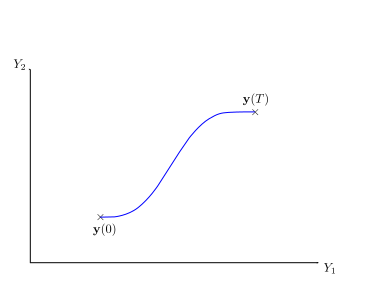
\includegraphics[scale=1]{img/state_transition.pdf}
	\caption{A feasible state transition from $\mathbf{y}(t_0)$ to $\mathbf{y}(t_{end})$}
	\label{fig:state_transition}
\end{figure}
A simple, but straight forward approach for a reference trajectory $\mathbf{y}_d(t)$ is a piecewise-defined function:
\begin{align}
\label{eq:14}
\mathbf{y}_d(t) = \begin{cases} \mathbf{y}(t_0) &\textrm{if } t<t_0 \\ \mathbf{y}(t_0) + (\mathbf{y}(t_{end})-\mathbf{y}(t_0))\varphi_\gamma\left(\frac{t-t_0}{t_{end}-t_0}\right) &\textrm{if } t \in [t_0, t_{end}] \\ \mathbf{y}(t_{end}) &\textrm{if } t>T\end{cases}
\end{align}
$\tau \rightarrow \varphi_\gamma(\tau)$ is a protoype function, where $\gamma$ indicates how often $\varphi_\gamma(\tau)$ is continuously differentiable. The function has to meet the following conditions, such that the reference trajectory is feasible:
\begin{subequations}
\label{eq:15}
\begin{align}
\varphi_\gamma(0)=0 \quad \varphi^{(j)}_\gamma(0)=0 \quad j = 1,...,\gamma \\
\varphi_\gamma(1)=1 \quad \varphi^{(j)}_\gamma(1)=0 \quad j = 1,...,\gamma 
\end{align}
\end{subequations}
An approach for the derivative of $\varphi_\gamma(\tau)$, which meets the conditions \eqref{eq:15} is:
\begin{align}
\frac{\d \varphi_\gamma(\tau)}{\d \tau} = \alpha \frac{\tau^{\gamma}}{\gamma!}\frac{(1-\tau)^{\gamma}}{\gamma!}
\end{align}
Integration leads to:
\begin{align}
\varphi_\gamma(\tau) = \alpha \int_0^\tau\frac{\tilde{\tau}^{\gamma}}{\gamma!}\frac{(1-\tilde{\tau})^{\gamma}}{\gamma!} \d \tilde{\tau}
\end{align}
After $\gamma$ partial integrations we get:
\begin{align*}
\varphi_\gamma(\tau)= \frac{\alpha}{(\gamma!)^2} \sum_{k=0}^{\gamma} \binom{\gamma}{k} \frac{(-1)^k\tau^{\gamma+k+1}}{(\gamma+k+1)}
\end{align*}
To solve for the unknown $\alpha$, we use the condition $\varphi_\gamma(1)\overset{!}{=}1$:
\begin{align*}
\varphi_\gamma(1)= &\frac{\alpha}{(\gamma!)^2} \sum_{k=0}^{\gamma} \binom{\gamma}{k} \frac{(-1)^k}{(\gamma+k+1)} \overset{!}{=} 1 \\
\Leftrightarrow \quad & \alpha = (2\gamma+1)!
\end{align*}
Finally we can define the prototype function:
\begin{align}
\varphi_\gamma(\tau)= \frac{(2\gamma+1)!}{(\gamma!)^2} \sum_{k=0}^{\gamma} \binom{\gamma}{k} \frac{(-1)^k\tau^{\gamma+k+1}}{(\gamma+k+1)}
\end{align}
and it's $n$-th derivative:
\begin{align}
\frac{\d^n }{\d \tau^n}\varphi_\gamma(\tau)=\varphi_\gamma^{(n)}(\tau)= \frac{(2\gamma+1)!}{(\gamma!)^2} \sum_{k=0}^{\gamma} \left(\binom{\gamma}{k} \frac{(-1)^k\tau^{\gamma+k-n+1}}{(\gamma+k+1)}\prod_{i=1}^n(\gamma+k-i+2)\right)
\end{align}
In the last step we can derive the $n$-th derivative of \eqref{eq:14} $(n=1,...,\gamma$).
\begin{align}
\frac{\d^n}{\d t^n}\mathbf{y}_d(t) = \begin{cases} \mathbf{y}^{(n)}(t_0) & \textrm{if } t<t_0 \\ \mathbf{y}^{(n)} + \sum_{i=0}^{n}\binom{n}{i}(\mathbf{y}^{(n-i)}(t_{end})-\mathbf{y}^{(n-i)}(t_0))\left(\frac{1}{t_{end}-t_0}\right)^i\varphi_\gamma^{(i)}\left(\frac{t-t_0}{t_{end}-t_0}\right) &\textrm{if } t \in [t_0, t_{end}] \\ \mathbf{y}^{(n)}(t_{end})&\textrm{if } t>T\end{cases}
\end{align}
%\newpage
%\subsection{Implementation of the controller in \py}
%\centering{\textcolor{red}{work in progress}}
%\subsection{Plotresults}
\end{document}
